\documentclass[a4paper,11pt,oneside]{book}

% PACCHETTI
\usepackage{hyperref}           % hyperlinks
\usepackage{tabto}              % strumento per inserire tab nel testo
\usepackage[                    % geometria della pagina
    a4paper,
    inner=2cm,
    outer=3cm,
    top=3cm,
    bottom=3cm,
    bindingoffset=1.2cm,
    headheight=14pt
]{geometry}
\usepackage[utf8]{inputenc}     % 3 pacchetti per l'italiano
\usepackage[italian]{babel}
\usepackage[T1]{fontenc}
\usepackage{titlesec}           % custom chapter titles

\usepackage{fancyhdr}
\usepackage{multicol}
\usepackage[arrowdel]{physics} 
\usepackage{amsmath}
\usepackage{tikz}

\usepackage{graphicx}           % IMMAGINI
\graphicspath{ {./images/} }
\usepackage{wrapfig}

\usepackage{csquotes}
\usepackage{caption}

% INFORMAZIONI SUL DOCUMENTO
\title{\Large{\textbf{Fisica 1}}}
\author{Enrico Bragastini}
\titleformat{\chapter}[display]{\normalfont\bfseries}{}{0pt}{\LARGE}


% CONTENUTO
\begin{document}
\pagestyle{fancy}
\fancyhf{}
\rhead{}
\lhead{\nouppercase\leftmark}
\cfoot{\thepage}
\frontmatter

% Prima pagina - Titolo
\maketitle
\tableofcontents

\mainmatter
\chapter{Nozioni di base}
\section{Misura di una grandezza}
Una \textbf{grandezza fisica} è la proprietà di un fenomeno, corpo o sostanza, che può essere espressa
quantitativamente mediante un numero e un riferimento.

\noindent La misura di una grandezza può avvenire con due modalità:
\begin{itemize}
    \item Mediante un dispositivo sperimentale
    \item Confronto con un'altra grandezza omogenea di riferimento e costante
\end{itemize}

\noindent L'espressione di una grandezza fisica avviene nella forma:
\begin{equation*}
    \text{Numero} + \text{\underline{\emph{Unità di misura}}}
\end{equation*}

\section{Grandezze fisiche fondamentali e derivate}
Possiamo distinguere le grandezze fisiche in \underline{fondamentali} e \underline{derivate}.

\noindent Le \textbf{grandezze fisiche fondamentali} sono:
\begin{itemize}
    \item Lunghezza                 \tabto{7cm} [L]
    \item Massa                     \tabto{7cm}  [M]
    \item Tempo                     \tabto{7cm}  [t]
    \item Intensità Di Corrente     \tabto{7cm}  [i]
    \item Temperatura Assoluta      \tabto{7cm}  [T]
\end{itemize}

\noindent Le \textbf{grandezze fisiche derivate} sono grandezze che possono essere
espresse in forma di combinazioni matematiche delle grandezze fondamentali.
Alcuni esempi di grandezze derivate sono:
\begin{itemize}
    \begin{multicols}{2}
        \item Superficie
        \item Volume
        \item Velocità
        \item Accelerazione
        \item Forza
        \item Pressione
    \end{multicols}
\end{itemize}

\section{Sistemi di Unità di Misura}
\begin{center}
    \bgroup
    \def\arraystretch{1.5}
    \begin{tabular}{ |c| c c c c c|}
        \hline
        SISTEMA     & Lunghezza & Massa & Tempo & Corrente & Temperatura \\
        \hline
        MKS (s. i.) & m         & kg    & s     & A        & °K          \\
        \hline
        cgs         & cm        & g     & s     & A        & °K          \\
        \hline
    \end{tabular}
    \egroup
\end{center}

\subsection{Ulteriori Unità di Misura}
Esistono ulteriori sistemi di unità di misura che permettono di avere maggiore comodità
nelle misurazioni di particolari grandezze.
Se ne elencano alcuni:

\begin{enumerate}
    \item Lunghezza:    \tabto{3cm} Ångströms, Anno-Luce
    \item Tempo:        \tabto{3cm} Minuto, Ora
    \item Volume:       \tabto{3cm} Litro
    \item Velocità:     \tabto{3cm} Chilometro/Ora
    \item Pressione:    \tabto{3cm} Atmosfera, Millimetro di mercurio
    \item Energia:      \tabto{3cm} Elettrovolt, Chilovattora
\end{enumerate}

\section{Notazione Scientifica}
Per i numeri particolarmente grandi o piccoli risulta comodo rappresentarli
in \textbf{Notazione Scientifica} utilizzando le potenze del 10.

La notazione scientifica permette di scrivere un numero in cui compare una sequenza molto lunga di zeri in forma compatta.
In matematica si dice che un numero è scritto in notazione scientifica se è della forma $n\cdot10^e$

~\newline
\underline{Esempio:}
\begin{equation*}
    1,2 \cdot 10^5
\end{equation*}
Un numero in \emph{notazione scientifica} è quindi composto da:
\begin{itemize}
    \item Un numero compreso n tale che $1 \leq n < 10$
    \item Una potenza del 10 con esponente intero
\end{itemize}

\newpage
\section{Analisi Dimensionale}
Quando si è di fronte ad una formula fisica o si svolgono calcoli con grandezze fisiche e unità di misura,
per verificare la plausibilità della formula data e la consistenza
dei calcoli svolti si può ricorrere all'analisi dimensionale.

Eseguire l'analisi dimensionale di una formula, o più in generale di un'equazione fisica,
vuol dire ricavare le dimensioni di ognuno dei due membri allo scopo di verificare che esse coincidano:
se così non fosse ci sarebbe necessariamente qualcosa di sbagliato, perché avremmo a che fare con un'equazione
dimensionalmente non consistente.


\section{Sistemi di Coordinate}
Molti aspetti della fisica hanno in qualche modo a che fare con la descrizione di un punto dello spazio.
Ad esempio, la descrizione matematica del moto di un corpo richiede un metodo che descriva la successione
delle posizioni occupate dal corpo nel tempo.

\subsection{Coordinate cartesiane}
In due dimensioni questa descrizione può essere realizzata con l’uso di un sistema di \textbf{coordinate cartesiane}
in cui due assi perpendicolari si intersecano in un punto definito come punto origine.
Le coordinate cartesiane sono anche dette \emph{coordinate rettangolari}.
\begin{figure}[h]
    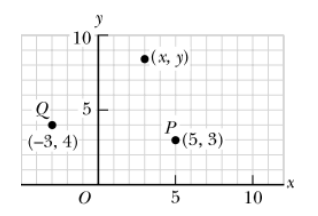
\includegraphics[scale=0.5]{coordinate_cartesiane}
    \centering
\end{figure}

\subsection{Coordinate scalari}
Talvolta è più conveniente rappresentare un punto in un piano tramite le sue \textbf{coordinate polari piane} $(r, \theta)$.

\begin{figure}[h]
    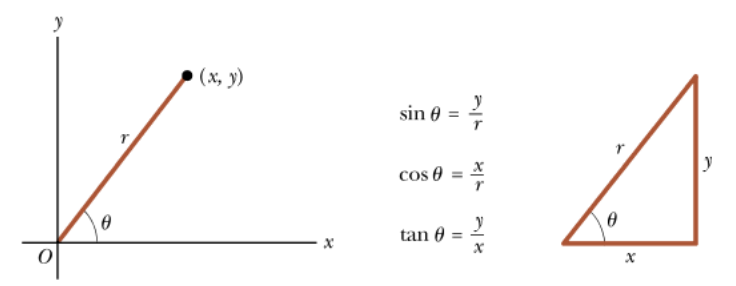
\includegraphics[scale=0.5]{coordinate_polari}
    \centering
\end{figure}
In questo sistema di coordinate polari, r è la distanza dall’origine al punto di coordinate
cartesiane $(x, y)$ e $\theta$ è l’angolo fra un asse fisso e la semiretta tracciata dall’origine al punto, generalmente
misurato in verso antiorario dall’asse x positivo.

\paragraph{Conversione delle coordinate} Partendo dalle coordinate polari, si possono ottenere le coordinate cartesiane
tramite le seguenti equazioni:
\begin{itemize}
    \item $x = r \cdot \cos{\theta}$
    \item $y = r \cdot \sin{\theta}$
\end{itemize}
Inoltre, sfruttando la trigonometria si possono ottenere queste altre informazioni:
\begin{itemize}
    \item $\tan{\theta} = \frac{y}{x}$
    \item $r = \sqrt{x^2 + y^2}$
\end{itemize}

\section{Grandezze scalari e grandezze vettoriali}

\subsection{Grandezza scalare}
Una \emph{grandezza scalare} è una grandezza che è specificata solamente da un valore con una certa unità di misura e non associata con una direzione.

Alcune grandezze scalari sono \emph{sempre positive}, come la massa e la velocità scalare.
Altre, come la temperatura, possono avere valori \emph{sia positivi che negativi}.
Per manipolare le quantità scalari si adoperano le \textbf{normali regole dell’aritmetica}.

\subsection{Grandezza vettoriale}
Una grandezza vettoriale è una grandezza che, per essere specificata,
ha bisogno sia di un numero con le sue unità di misura (\textbf{modulo del vettore}), sia di una \textbf{direzione orientata}.

Per rappresentare un vettore, si utilizza una lettera sormontata da una freccia come da esempio:
\begin{equation*}
    \vec{A}
\end{equation*}

\newpage
\section{Proprietà e operazioni con i vettori}
\subsection{Uguaglianza di due vettori}
Due vettori $\vec{A}$ e $\vec{B}$ sono \textbf{uguali} se sono uguali i loro \emph{moduli}, la \emph{direzione} e il \emph{verso}.
L'uguaglianza è \emph{indipendente dall'origine}, ovvero i vettori possono essere traslati sul grafico in base alla necessità
senza che venga persa la loro uguaglianza.
\begin{figure}[h]
    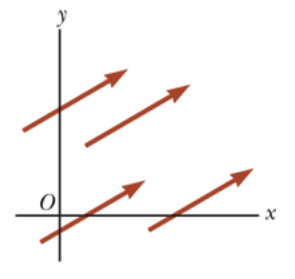
\includegraphics[scale=0.5]{uguaglianza_vettori}
    \centering
\end{figure}

\subsection{Somma tra vettori (metodo grafico)}
La somma tra vettori può essere svolta rapidamente in modo grafico.

In generale, se si vogliono sommare due spostamenti rappresentati dai due vettori $\vec{a}$ e $\vec{b}$ come di seguito rappresentato:
\begin{figure}[h]
    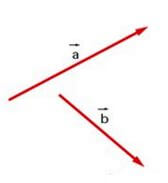
\includegraphics[scale=0.5]{vettori_da_sommare}
    \centering
\end{figure}

\paragraph{Metodo punta-coda:} Spostiamo uno dei due vettori in modo tale che la sua coda coincida con la punta del primo vettore.

~\newline
\noindent Riferendoci al nostro caso, spostiamo il vettore $\vec{b}$ vettore in modo tale che la sua coda coincida con la
punta del vettore $\vec{a}$, come di seguito rappresentato:
\begin{figure}[h]
    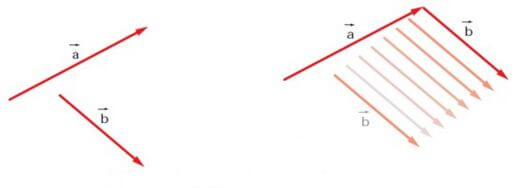
\includegraphics[scale=0.5]{punta_coda}
    \centering
\end{figure}

Come è possibile notare dalla figura precedente lo spostamento del vettore $\vec{b}$ deve essere effettuato in modo
tale che la freccia rimanga sempre parallela a se stessa.
Lo spostamento totale si ottiene unendo la coda del vettore $\vec{a}$ con la punta del vettore $\vec{a}$, come di seguito
rappresentato:
\begin{figure}[h]
    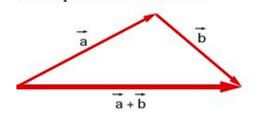
\includegraphics[scale=0.5]{vettori_sommati}
    \centering
\end{figure}

Si noti che in generale il modulo del vettore somma non è uguale alla somma dei moduli dei singoli spostamenti.

\subsection{Opposto di un vettore}
L'\textbf{opposto di un vettore} $\vec{A}$ è definito come il vettore che sommato a $\vec{A}$ permette di ottenere 0.
\begin{equation*}
    \vec{A} + (- \vec{A} ) = 0
\end{equation*}
Il vettore $(-\vec{A})$ è quindi un vettore che ha lo \textbf{stesso modulo} di $\vec{A}$, con la \textbf{stessa direzione} ma di \textbf{verso opposto}.

\subsection{Sottrazione tra vettori}
La \textbf{sottrazione tra vettori} si ottiene sfruttando la definizione di \emph{vettore opposto}.
Quindi, si vuole sottrarre il vettore $\vec{B}$ al vettore $\vec{A}$, basta \emph{sommarne l'opposto}.
\begin{equation*}
    \vec{A} - \vec{B} = \vec{A} + (- \vec{B})
\end{equation*}

\subsection{Prodotto tra un vettore e uno scalare}
\begin{itemize}
    \item Se un vettore $\vec{A}$ viene moltiplicato per una quantità scalare positiva $m$,
          allora il prodotto è $m\vec{A}$ e possiede la stessa direzione di A e modulo $mA$.
    \item Se un vettore $\vec{A}$ viene moltiplicato per una quantità scalare negativa $-m$,
          allora il prodotto è $-m\vec{A}$ e possiede direzione opposta di A e modulo $mA$.
\end{itemize}

\newpage
\section{Componenti di un vettore e vettori unitari}
\subsection{Componenti di un vettore}
Il metodo geometrico di somma vettoriale non è raccomandabile in quelle situazioni in cui si richiede una precisione elevata, oppure nei problemi in tre dimensioni.
Esiste un metodo per sommare i vettori che fa uso delle \emph{proiezioni dei vettori} lungo gli assi coordinati.
Queste proiezioni sono chiamate \textbf{componenti del vettore} o anche componenti rettangolari del vettore. Un vettore può essere descritto in modo completo dai suoi componenti.

Un vettore $\vec{A}$ può essere espresso come come \emph{somma di due vettori componenti}: $\vec{A_x}$, parallelo all'asse $x$, sommato a $\vec{A_y}$,
parallelo all'asse $y$.
\begin{figure}[h]
    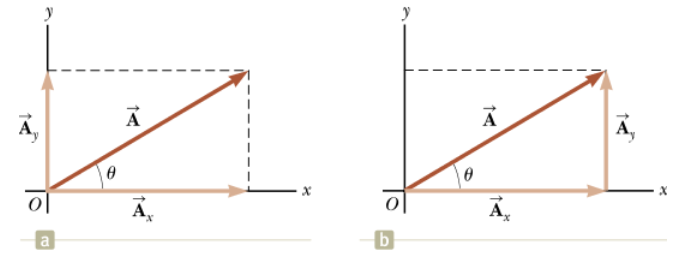
\includegraphics[scale=0.5]{vettori_componenti}
    \centering
\end{figure}

\noindent Si ottengono quindi le seguenti relazioni:
\begin{itemize}
    \item $\vec{A} = \vec{A_x} + \vec{A_y}$
    \item $\vec{A_x} = A \cos{\theta}$
    \item $\vec{A_y} = A \sin{\theta}$
    \item $A = \sqrt{A_x^2 + A_y^2}$
    \item $\theta = \tan[-1](\frac{A_y}{A_x})$
\end{itemize}
Nell’affrontare un problema fisico si può scegliere di specificare un vettore $\vec{A}$
per mezzo delle sue componenti $\vec{A_x}$ e $\vec{A_y}$ oppure per mezzo del suo modulo A e dell’angolo $\theta$.

\subsection{Vettori unitari}
Un \textbf{vettore unitario} è un \emph{vettore adimensionale} il cui modulo è esattamente 1.
I vettori unitari hanno l'unico scopo di indicare una direzione orientata e non hanno nessun altro significato fisico.
Il modulo dei vettori unitari è uguale a 1, ovvero $\abs*{\hat{i}} = \abs*{\hat{j}} = \abs*{\hat{k}} = 1$

Useremo i simboli $\hat{i}$, $\hat{j}$, e $\hat{k}$ per rappresentare i vettori unitari che puntano rispettivamente nelle direzioni positive x, y e z.

\newpage
\begin{figure}[h]
    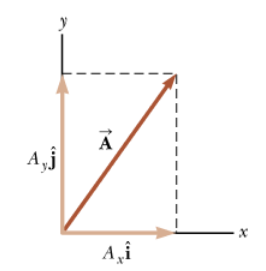
\includegraphics[scale=0.5]{vettori_unitari}
    \centering
\end{figure}
Consideriamo un vettore $\vec{A}$ che giace nel piano $xy$ come in figura.
Il prodotto della componente $A_x$ per il vettore unitario $\hat{i}$ è il vettore $\vec{A_x} = A_x \hat{i}$ parallelo all'asse delle $x$ e di modulo $\abs{A_x}$.
Analogamente, $\vec{A_y} = A_y \hat{j}$ è un vettore di modulo $\abs{A_y}$ parallelo all’asse $y$.
Così, nella notazione dei vettori unitari, il vettore $\vec{A}$ è
\begin{equation*}
    \vec{A} = A_x \hat{i} \cdot A_y \hat{j}
\end{equation*}

\subsection{Somma tra vettori (metodo con vettori unitari)}
Quando il metodo grafico non risulta sufficientemente accurato ci si può avvalere dell'utilizzo delle componenti dei vettori da sommare.

Si supponga di voler sommare il vettore $\vec{A}$ composto da $\vec{A_x}$ e da $\vec{A_y}$ al vettore $\vec{B}$
composto da $\vec{B_x}$ e da $\vec{B_y}$.

\begin{figure}[h]
    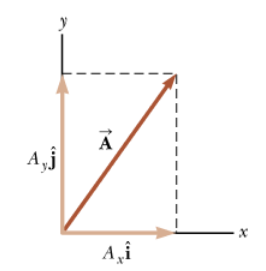
\includegraphics[scale=0.5]{vettori_unitari}
    \centering
\end{figure}

\noindent Per effettuare questa somma basta sommare separatamente le componenti $x$ e $y$. Il vettore risultante $\vec{R} = \vec{A} + \vec{B}$
si ottiene con:
\begin{equation*}
    \vec{R} = (A_x \hat{i} + A_y \hat{j}) + (B_x \hat{i} + B_y \hat{j})
\end{equation*}
ovvero
\begin{equation*}
    \vec{R} = (A_x+ B_x) \hat{i} + (A_y + B_y) \hat{j}
\end{equation*}

~\newline
\noindent Il vettore ottenuto può essere a sua volta visto come $\vec{R} = R_x \hat{i} + R_y \hat{j}$.



\chapter{Cinematica}

La \textbf{Cinematica} è un ramo della \textbf{meccanica classica} che si occupa di descrivere quantitativamente il moto dei corpi, indipendentemente dalle cause del moto stesso.

\section{Moto in una dimensione}

\paragraph{Punto materiale}
Nello studio del moto traslatorio utilizziamo il modello \textbf{punto materiale} e descriviamo il moto di un corpo approssimandolo ad
“una particella” senza considerare le sue dimensioni reali.

In generale un punto materiale è quel corpo che \emph{ha una massa} ma \emph{ha dimensioni infinitesimali}.

\section{Posizione, spostamento e distanza}

\paragraph{Posizione} Indichiamo come posizione il punto occupato \emph{istante per istante} dal punto materiale oggetto di studio.
Un corpo è considerato \emph{in moto} se la sua posizione cambia con il passare del tempo.

\paragraph{Spostamento} Lo spostamento, indicato con $\Delta x$\footnote{La lettera greca $\Delta$ indica in generale una \emph{variazione}} è definito come la variazione della sua posizione in un certo intervallo di tempo.

Se da $x_i$ il punto materiale raggiunge la posizione $x_f$ il suo spostamento è definito come la posizione finale meno la posizione iniziale:
\begin{equation*}
    \Delta x = x_f - x_i
\end{equation*}
Lo spostamento è una \emph{grandeza vettoriale}, ma sul moto rettilineo è possibile considerarlo come una \emph{lunghezza scalare}.

\paragraph{Distanza percorsa}
La distanza percorsa \emph{non è lo spostamento}. La distanza indica la lunghezza del cammino percorso da una particella.

Supponiamo che un'automobile parta dal punto $A$, arrivi al punto $B$ e poi ritorni al punto $A$. In questo caso abbiamo che lo spostamento
è nullo, infatti $x_i = x_f$, ovvero $\Delta x = 0$. Mentre la distanza percorsa corrisponde a $2 (B-A)$.

\section{Velocità media e istantanea}

\paragraph{Velocità media}
La \textbf{velocità media}, $v_{m}$ di un punto materiale, è definita come il rapporto tra lo spostamento $\Delta x$ del punto materiale
e l’intervallo di tempo $\Delta t$ durante il quale lo spostamento è avvenuto:
\begin{equation*}
    v_{x,media} \equiv \frac{\Delta x}{\Delta t}
\end{equation*}

\begin{itemize}
    \item L'unità di misura è: $\frac{m}{s}$
    \item Se $\Delta x > 0$ (spostamento nel verso positivo), allora $v_m > 0$.
    \item Se $\Delta x < 0$ (spostamento nel verso negativo), allora $v_m < 0$
\end{itemize}

\paragraph{Velocità media scalare}
La velocità scalare media $v_{media}$ di un punto materiale, una quantità scalare, è definita come il rapporto
fra la distanza totale $d$ percorsa e l’intervallo di tempo impiegato a percorrerla:
\begin{equation*}
    v_{m} \equiv \frac{d}{\Delta t}
\end{equation*}

\paragraph{Velocità istantanea}
La velocità istantanea $v_x$ di un corpo in un determinato istante di tempo $t$ è uguale al valore limite del rapporto $\frac{\Delta x}{\Delta t}$
quando $\Delta t$ tende a $0$. Nel linguaggio del calcolo differenziale questo limite è la derivata di x rispetto a t:
\begin{equation*}
    v_x \equiv \lim_{\Delta t \to 0} \frac{\Delta x}{\Delta t} = \frac{dx}{dt}
\end{equation*}

~\newline
\underline{Esempio:} \newline
Espressione analitica dello spostamento di un punto materiale: $x=-4t + 2t^2$
Calcolo della velocità istantanea a $t = 2,5s$
\begin{align*}
    x             & = -4t + 2t^2 \\
    \frac{dx}{dt} & = -4 + 4t    \\
    v_x           & = 6 \; m/s
\end{align*}

\section{Moto Rettilineo Uniforme}
Un corpo si muove con \textbf{moto rettilineo uniforme} quando si sposta lungo una retta con velocità costante.

Basandoci su questa definizione si possono ricavare le seguenti equazioni:
\begin{itemize}
    \item $v_x = \text{costante}$
    \item $v_{x,media} = v_x$
    \item $v_x = \frac{\Delta x}{\Delta t} = \frac{x_f - x_i}{t_f - t_i}$
    \item $x_f = x_i + \frac{v_x(t_f - t_i)}{v_x \Delta t}$, scegliendo \tiny $\begin{aligned} t_i&=0 \\ t_f&=t \end{aligned}$ \normalsize otteniamo $x_f = x_i + v_x \cdot t$
\end{itemize}

\section{Accelerazione media e istantanea}

\paragraph{Accelerazione media} Quando la velocità cambia nel tempo, si dice che la particella sta accelerando.
L’accelerazione media $a_{x,media}$ del punto materiale è definita come la variazione della velocità
$\Delta v_x$ divisa per l’intervallo di tempo $\Delta t$ in cui avviene la variazione:
\begin{equation*}
    a_{x,media} \equiv \frac{\Delta v_x}{\Delta t} = \frac{v_{xf} - v_{xi}}{t_f - t_i   }
\end{equation*}
L'unità di misura dell'accelerazione è $m/s^2$

\paragraph{Accelerazione instantanea} Si definisce l'accelerazione istantanea come il limite dell'accelerazione
media quando $\Delta t$ tende a zero.
\begin{equation*}
    a_{x,media} \equiv \lim_{\Delta t \to 0} \frac{\Delta v_x}{\Delta t} = \frac{dv_x}{dt} = \frac{d}{dt} (\frac{dx}{dt}) = \frac{d^2x}{dt^2}
\end{equation*}
L’accelerazione istantanea è la derivata della velocità rispetto al tempo che è anche la pendenza della curva del grafico velocità–tempo.

\section{Moto rettilineo uniformemente accelerato}
Nel caso del \textbf{moto rettilineo uniformemente accelerato}, il moto del \emph{punto materiale} avviene con \emph{accelerazione costante}.

~\newline
\noindent Se il moto avviene con accelerazione costante, allora la velocità media e la velocità istantanea coincidono.
\begin{equation*}
    a_x = \frac{v_{xf}-v_{xi}}{t_f-t_i}
\end{equation*}
Supponendo $t_i = 0$ otteniamo $a_x = \frac{v_{xf}-v_{xi}}{t}$ e quindi $v_{xf} = v_{xi} + a_x t$ (per $a_x$ costante)

Poiché la velocità varia linearmente con il tempo, la velocità media in un intervallo di tempo
arbitrario è uguale alla \emph{media aritmetica} della velocità iniziale $v_{xi}$ e della velocità finale $v_{xf}$:
\begin{equation*}
    v_{media} = \frac{v_{xi} + v_{xf}}{2} = \frac{1}{2} (v_{xi} + v_{xf}) \; \; \text{(per } a_{x} \text{ costante)}
\end{equation*}

Ora, ricordando che $\Delta x = x_f - x_i$ e che $\Delta t = t_f - 0 = t$, si ottiene:
\begin{equation*}
    x_f - x_i = v_{media} t = \frac{1}{2} (v_{xi} + v_{xf}) t
\end{equation*}
\begin{align*}
    x_f & = x_i + \frac{1}{2} (v_{xi} + v_{xf}) t                                         \\
    x_f & = x_i + \frac{1}{2} [v_{xi} + (v_{xi} + a_x t)] t                               \\
    x_f & = x_i + v_{xi} t + \frac{1}{2} a_x t^2 \; \; \text{(per } a_x \text{ costante)}
\end{align*}
Si può infine ottenere un’espressione per la velocità finale che non contiene il tempo:
\begin{equation*}
    v_{xf}^2 = v_{xi}^2 + 2ax(x_f - x_i)
\end{equation*}

\subsection{Corpi in caduta libera}
È un fatto ben noto che vicino alla superficie della Terra e senza la resistenza dell’aria,
tutti i corpi sotto l’influenza della gravità terrestre cadono verso la Terra con la \textbf{stessa accelerazione costante}.

Indicheremo il modulo dell’accelerazione di caduta libera, detta anche accelerazione di gravità con il simbolo $g$.
Sulla superficie della Terra, il valore di $g$ è approssimativamente 9.80 $m/s^2$.

\section{Moto in due dimensioni}
A differenza del moto in una sola dimensione, nel \emph{moto a due dimensioni}, le posizioni di inizio e di fine dello spostamento
di un punto materiale sono \textbf{grandezze vettoriali} e sono indicate da $\vec{r_i}$ e $\vec{r_f}$.

La posizione è quindi descritta dal \emph{vettore} $\vec{r}$. Lo spostamento del punto materiale è indicato con $\Delta \vec{r} = \vec{r_f}-\vec{r_i}$.

\paragraph{Velocità media}
La velocità media è definita come:
\begin{equation*}
    \vec{v}_{media} \equiv \frac{\Delta \vec{r}}{\Delta t}
\end{equation*}
La direzione e il verso di $\vec{v}_{media}$ sono le stesse di $\Delta \vec{r}$ in quanto $\Delta t$ è uno scalare.

\paragraph{Velocità istantanea}
La velocità istantanea è definita come:
\begin{equation*}
    \vec{v} \equiv \lim_{\Delta t \to 0} \frac{\Delta \vec{r}}{\Delta t} = \frac{d \vec{r}}{dt}
\end{equation*}
La velocità istantanea è la \emph{derivata} del vettore posizione rispetto al
tempo. La direzione del vettore velocità istantanea in un punto è quella della retta tangente alla traiettoria in quel punto ed è orientata nel verso del moto.

\paragraph{Accelerazione media}
Conoscendo la velocità in ciascuno dei due punti è possibile determinare l'accelerazione media:
\begin{equation*}
    \vec{a}_{media} \equiv \frac{\Delta \vec{v}}{\Delta t} = \frac{\vec{v_f} - \vec{v_i}}{t_f - t_i}
\end{equation*}

\paragraph{Accelerazione istantanea}
Dall'accelerazione media è possibile ricavare l'accelerazione istantanea:
\begin{equation*}
    \vec{a} \equiv \lim_{\Delta t \to 0} \frac{\Delta \vec{v}}{\Delta t} = \frac{d\vec{v}}{dt}
\end{equation*}

\newpage
\subsection{Moto in due dimensioni con accelerazione costante}
Il moto in due dimensioni può essere modellizzato come \emph{due moti indipendenti} lungo
ciascuna delle due direzioni ortogonali che possono essere associate agli \emph{assi $x$ e $y$}.
Qualunque azione in direzione $x$ non influenza il moto in direzione $y$ e viceversa.

\begin{figure}[h]
    \centering
    \begin{tikzpicture}
        \draw[thin,gray!40] (0,0) grid (4,4);
        \draw[<->] (0,0)--(4,0) node[right]{$x$};
        \draw[<->] (0,0)--(0,4) node[above]{$y$};
        \draw[line width=2pt,black,-stealth](0,0)--(2.5,2.5) node[anchor=south west]{$P(x,y)$};
        \draw[line width=1pt,black,-stealth](0,0)--(0,2.5) node[anchor=north east]{$y \hat{j}$};
        \draw[line width=1pt,black,-stealth](0,0)--(2.5,0) node[anchor=north east]{$x \hat{i}$};

        \draw[dashed,line width=0.5pt,black,](0,2.5)--(2.5,2.5);
        \draw[dashed,line width=0.5pt,black,](2.5,0)--(2.5,2.5);
    \end{tikzpicture}
\end{figure}
\noindent Il \textbf{vettore posizione} per un punto materiale che si muove nel piano $xy$ può essere scritto come
\begin{equation*}
    \vec{r} = x\hat{i} + y\hat{j}
\end{equation*}
Se il vettore posizione è noto, la \textbf{velocità} può essere ricavata:
\begin{equation*}
    \vec{v} = \frac{d\vec{r}}{dt} = \frac{dx}{dt}\hat{i}+\frac{dy}{dt}\hat{j} = v_x \hat{i} + v_y \hat{j}
\end{equation*}
Essendo l'\textbf{accelerazione costante}, anche $a_x$ e $a_y$ sono costanti.

\noindent Sostituendo $v_{xf} = v_{xi} + a_x t$ e $v_{yf} = v_{yi} + a_y t$ alla formula della velocità si ottiene:
\begin{align*}
    v_f & = (v_{xi} + a_x t)\hat{i} + (v_{yi} + a_y t)\hat{j}            \\
        & = (v_{xi}\hat{i} + v_{yi}\hat{j}) + (a_x\hat{i} + a_y\hat{j})t \\
        & = v_i + at
\end{align*}

\noindent Analogamente le coordinate $x_f$ e $y_f$ sono date da:
\begin{align*}
    x_f & = x_i + v_{xi}t + \frac{1}{2}a_xt^2 & y_f & = v_i + v_{yi} + \frac{1}{2}a_yt^2
\end{align*}

\noindent Sostituendole nella formula del vettore posizione si ottiene:
\begin{align*}
    \vec{r}_f & = x\hat{i} + y\hat{j}                                                                                            \\
              & = (x_i + v_{xi}t + \frac{1}{2}a_xt^2)\hat{i} + (v_i + v_{yi} + \frac{1}{2}a_yt^2)\hat{j}                         \\
              & = (x_i \hat{i} + y_i \hat{j}) + (v_{xi} \hat{i} + v_{yi} \hat{j})t + \frac{1}{2} (a_x \hat{i} + a_y \hat{j}) t^2 \\
              & = \vec{r}_i + \vec{v}_i t + \frac{1}{2} \vec{a} t^2
\end{align*}

\subsection{Moto dei proiettili}
Il moto dei proiettili (moto parabolico) può essere analizzato mediante due ipotesi:
\begin{enumerate}
    \item l’accelerazione di caduta libera si mantiene costante per tutto il moto ed è diretta verso il basso
    \item l’effetto della resistenza dell’aria è trascurabile
\end{enumerate}
Sotto queste ipotesi, la traiettoria del proiettile è \emph{sempre una parabola}.

\begin{figure*}[h]
    \centering
    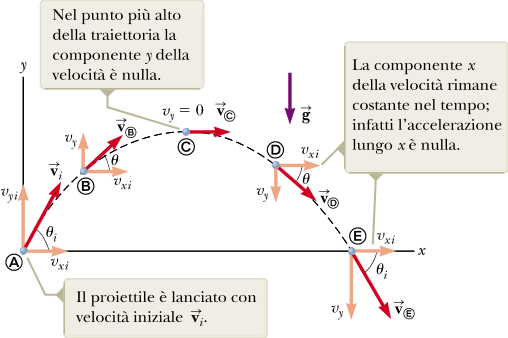
\includegraphics[scale=0.5]{moto_proiettili}
\end{figure*}

Il moto del proiettile è considerabile con accelerazione orizzontale $a_x = 0$,
mentre l'accelerazione verticale è costante: $\vec{a} = \vec{g}$. L'espressione del vettore posizione del proiettile è quindi pari a:
\begin{equation*}
    \vec{r}_f = \vec{r}_i + \vec{v}_i t + \frac{1}{2} \vec{g}t^2
\end{equation*}
dove le due componenti di $\vec{v}_i$ sono:
\begin{align*}
    v_{xi} & = v_i \cos{\theta_i} & v_{yi} & = v_i \sin{\theta_i}
\end{align*}

Tenendo a mente che il moto del proiettile è la sovrapposizione di un punto materiale con velocità orizzontale costante
\begin{equation*}
    x_f = x_i + v_{xi}t
\end{equation*}
e un punto materiale
con accelerazione verticale costante ($a_y = -g$), otteniamo le seguenti relazioni:
\begin{itemize}
    \item $v_{yf} = v_{yi} - gt$
    \item $v_{y,media} = \frac{v_{yi} + v_{yf}}{2}$
    \item $y_f = y_i + \frac{1}{2} (v_{yi} + v_{yf})t$
    \item $y_f = y_i + v_{yi}t - \frac{1}{2} gt$
    \item $v_{yf}^2 = v_{yi}^2 -2g(y_f - y_i)$
\end{itemize}

\paragraph{Altezza massima}
L'altezza massima $h_{max}$ raggiunta dal corpo lanciato è determinabile notando che nel \emph{picco} la velocità verticale si annulla $v_y = 0$
\begin{equation*}
    v_{yf} = v_{yi} - gt \; \rightarrow \; 0 = v_i \sin{\theta_i} -gt
\end{equation*}
\begin{equation*}
    t = \frac{v_i \sin{\theta_i}}{g} \;\;\; \text{(tempo per raggiungere } h_{max} \text{)}
\end{equation*}
Possiamo utilizzare questa espressione del tempo per calcolare l'altezza massima raggiunta. Partendo dalla precedente espressione per il calcolo di
$y_f$ si sostituisce t con l'espressione appena trovata e $y_f$ diventa l'altezza $h_{max}$
\begin{align*}
    y_f = y_i + v_{yi}t - \tfrac{1}{2}gt^2 \;\; \rightarrow \;\; h_{max} & = 0 + (v_i \sin{\theta_i})\tfrac{v_i \sin{\theta_i}}{g} - \tfrac{1}{2}g(\tfrac{v_i \sin{\theta_i}}{g})^2 \\
    h_{max}                                                              & = \frac{v_i^2 \sin^2{\theta_i}}{2g}
\end{align*}

\paragraph{Gittata}
La gittata $R$ è la distanza orizzontale percorsa dal proiettile in un \emph{tempo doppio} di quello necessario a raggiungere l'altezza massima.
\begin{align*}
    x_f & = x_i + v_{xi}t                 & R & = v_{xi}t = (v_i \cos{\theta_i})2t                                                                     \\
    t   & = \tfrac{v_i \sin{\theta_i}}{g} & R & = (v_i \cos{\theta_i}) \tfrac{2v_i \sin{\theta_i}}{g} = \tfrac{2v_i^2 \sin{\theta_i}\cos{\theta_i}}{g}
\end{align*}
Poiché vale la relazione $2\sin{\theta_i}\cos{\theta_i} = \sin{2\theta}$, si può scrivere:
\begin{equation*}
    R = \frac{v_i^2 \sin{2\theta_i}}{g}
\end{equation*}


\section{Moto Circolare Uniforme}
Il \emph{moto circolare} è uno dei moti semplici studiati dalla fisica e dalla cinematica, e consiste in un moto di un punto materiale lungo una circonferenza. 

Se il \textbf{moto circolare} è \textbf{uniforme} significa che \textbf{è costante il vettore velocità angolare}, cioè si ha \textbf{velocità lineare costante in modulo}. 
Poiché comune in molte situazioni fisiche, questo tipo di moto viene schematizzato in un modello di analisi, detto \textbf{punto materiale in moto circolare uniforme}.

Il \textbf{vettore velocità}, che è sempre \textbf{tangente alla traiettoria}, è \textbf{perpendicolare al raggio} della traiettoria circolare. Quindi la direzione del vettore velocità cambia continuamente.

In un moto circolare uniforme il \textbf{vettore accelerazione} può avere solamente un componente \textbf{perpendicolare alla traiettoria}, ovvero \emph{diretto verso il centro della circonferenza}.
\begin{figure*}[h]
    \centering
    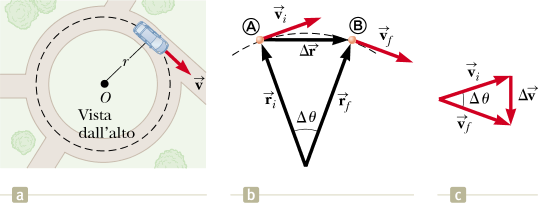
\includegraphics[scale=0.5]{moto_circolare_uniforme}    
\end{figure*}

\paragraph{Accelerazione media}
Partendo dall'equazione $\vec{a}_{media} = \tfrac{\Delta \vec{v}}{\Delta t}$ e conoscendo la relazione tra le lunghezze nei due triangoli delle figure
\begin{equation*}
    \tfrac{\abs{\Delta \vec{v}}}{v} = \tfrac{\abs{\Delta \vec{r}}}{r}
\end{equation*}
è possibile calcolare il modulo dell'accelerazione media nell'intervallo di tempo in cui avviene lo spostamento:
\begin{equation*}
    \abs{\vec{a}_{media}} = \frac{\abs{\Delta \vec{v}}}{\abs{\Delta t}} = \frac{v}{r}\frac{\abs{\Delta \vec{r}}}{\Delta t}
\end{equation*}
Infine, passando al limite per $\Delta t \to 0$, si ottiene per il modulo dell'accelerazione:
\begin{equation*}
    a_c = \frac{v^2}{r}
\end{equation*}
Questo tipo di accelerazione è chiamata \textbf{accelerazione centripeta}.

\paragraph{Periodo}
È conveniente descrivere il moto circolare uniforme di un punto materiale su una circonferenza di raggio $r$ usando come parametro il \textbf{periodo $T$}, 
definito come l’intervallo di tempo necessario perché il punto compia una \emph{rivoluzione} completa. Nell’intervallo di tempo $T$ il punto percorre la circonferenza 
di lunghezza $2\pi r$. Ne segue che la velocità costante è uguale alla lunghezza della circonferenza divisa per il periodo, e cioè $v = \tfrac{2\pi r}{T}$ e, da questa:
\begin{equation*}
    T = \frac{2\pi r}{v}
\end{equation*}

\paragraph{Velocità angolare}
Il reciproco del periodo è la \emph{frequenza}, e si misura in giri al secondo. Poiché un giro completo del punto materiale corrisponde ad una rotazione di $2\pi$ radianti,
il prodotto tra $2\pi$ e la frequenza dà la \textbf{velocità angolare $\omega$} del punto materiale, che si misura in radianti/s:
\begin{equation*}
    \omega = \frac{2\pi}{T}
\end{equation*}

\paragraph{Rapporto tra velocità angolare e velocità}
Combinando l'espressione della \emph{velocità angolare} con quella del \emph{periodo} è possibile trovare una relazione tra la velocità angolare e la velocità con cui il 
punto si muove sulla traiettoria circolare:
\begin{equation*}
    \omega = 2\pi \left (\frac{v}{2\pi r} \right)  = \frac{v}{r} \;\; \rightarrow \;\; v = r\omega
\end{equation*}
Fissata la velocità angolare, \textbf{la velocità aumenta all'aumentare del raggio}.

È possibile esprimere l'accelerazione centripeta in moto circolare uniforme in termini della velocità angolare:
\begin{align*}
    a_c &= \frac{(r\omega)^2}{r} & a_c &= r\omega^2
\end{align*}


\chapter{Dinamica}
In fisica, la dinamica è il ramo della meccanica newtoniana che si occupa dello \emph{studio del moto dei corpi a partire dalle sue cause}, le \textbf{forze}
o, in termini più concreti, delle circostanze che lo determinano e lo modificano nel tempo e nello spazio del suo sistema di riferimento.

\section{Concetto di forza}
Le \textbf{forze} sono definite come le cause che provocano un cambiamento nel moto del corpo, nella velocità del corpo.
Si possono distinguere le forze in due categorie:
\begin{enumerate}
    \item \textbf{Forze di contatto}, ovvero forze che si esercitano attraverso il contatto fisico tra due oggetti.
    \item \textbf{Forze di campo}, ovvero le forze che che non richiedono il contatto fisico tra gli oggetti, come la forza gravitazionale, la forza elettrica o la forza magnetica.
\end{enumerate}
Tuttavia, se vengono esaminate a livello atomico, tutte le forze, che classifichiamo come forze di contatto, sono in realtà dovute
alle forze elettriche (forze di campo). Di fatto tutte le forze conosciute in natura sono \emph{forze di campo}:
\begin{enumerate}
    \item Attrazione gravitazionale
    \item Forze elettromagnetiche
    \item Forze nucleari forti tra particelle subatomiche
    \item Forze nucleari deboli (in processi di decadimento radioattivo)
\end{enumerate}

\noindent Le forze hanno una \textbf{natura vettoriale}. È possibile infatti provare sperimentalmente che le forze agiscono secondo una
natura vettoriale e di conseguenza è necessario utilizzare le regole della \emph{somma di vettori} per ottenere la forza risultante su di un corpo.

\newpage
\begin{figure*}[h]
    \centering
    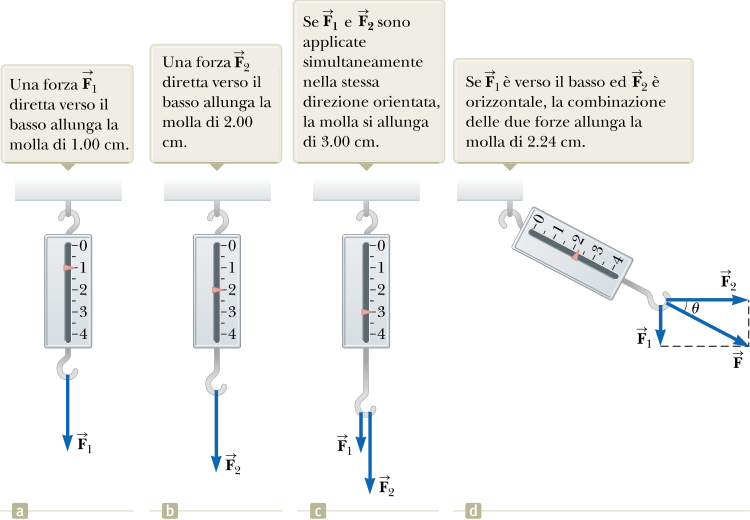
\includegraphics[scale=0.5]{natura_vettoriale_forze}
\end{figure*}
Come mostrato nella nel punto \emph{d} della figura, le due forze vengono applicate simultaneamente con $\vec{F}_1$ verticalmente verso
il basso e $\vec{F}_2$ orizzontalmente. In questo caso, l’indicatore indicherà \emph{2.24 cm}. La forza $\vec{F}$ che produce
la stessa lettura della somma dei due vettori $\vec{F}_1$ e $\vec{F}_2$. In altre parole, $\abs{\vec{F}_1} = \sqrt{F_1^2 + F_2^2} = 2.24$
unità e la sua direzione è $\theta = \tan^{-1} (-0.500) = -26.6$°

\paragraph{Dinamometro}
Il dinamometro è uno strumento di misura utilizzato in meccanica per determinare l'entità di una forza ad esso applicata.
Il meccanismo di misurazione utilizza il principio della legge di Hooke, per il quale la deformazione di un materiale elastico è direttamente proporzionale alla forza applicata al materiale stesso.

\newpage
\section{Prima legge di Newton - principio d'Inerzia}
La \textbf{prima legge di Newton} del moto, che viene spesso chiamata \textbf{legge d’inerzia},
definisce una particolare classe di sistemi di riferimento detti \textbf{sistemi inerziali}.
Questa legge può essere espressa nel seguente modo:
\begin{displayquote}
    \centering
    Se un corpo non interagisce con altri corpi, si può trovare un sistema di riferimento nel quale la sua accelerazione è nulla.
\end{displayquote}
Un tale sistema di riferimento viene chiamato \textbf{sistema di riferimento inerziale}.
Ogni sistema di riferimento che si muove a velocità costante rispetto ad un sistema di riferimento inerziale, è esso stesso un \emph{sistema inerziale}.

~\newline
Per i nostri scopi possiamo considerare anche la \emph{Terra come un sistema inerziale}. La Terra in realtà non è un sistema inerziale a causa del suo moto
orbitale intorno al Sole e del suo moto di rotazione intorno all’asse terrestre.
Queste accelerazioni hanno comunque valori piccoli rispetto a $g$ e possono spesso essere trascurate.

\noindent È possibile riformulare la \emph{prima legge di Newton} in un modo più pratico:
\begin{displayquote}
    \centering
    In assenza di forze esterne e se osservato da un sistema di riferimento inerziale, un corpo in quiete rimane in quiete ed un
    corpo in moto rimane in moto (con moto rettilineo uniforme).
\end{displayquote}

\paragraph{Inerzia} È possibile definire l'\emph{inerzia} come la \emph{tendenza di un corpo a non modificare il suo stato di moto}.

\subsection{Massa}
Quantitativamente il concetto di \emph{inerzia} viene quantificato dalla \textbf{massa}. La massa è la proprietà (scalare) di un corpo che misura
quanta resistenza un corpo offre al cambiamento di velocità. È una delle grandezze fondamentali.

L'unità di misura della massa \emph{m} è il \emph{kg}.

\paragraph{Rapporto massa-accelerazione}
Tra le due grandezze vi è un rapporto \emph{inversamente proporzionale}.

Si supponga di applicare una stessa forza $\vec{F}$ a due masse diverse $m_1$ e $m_2$, andando a misurare le accelerazioni $a_1$ e $a_2$ che la forza ha provocato.
Si verificherà la seguente relazione: $\frac{m_1}{m_2} \equiv \frac{a_1}{a_2}$

\newpage
\section{Seconda legge di Newton}
La \textbf{seconda legge di Newton} risponde alla domanda: che cosa succede ad un corpo se su di esso agiscono una o più forze?
\begin{itemize}
    \item L’accelerazione di un corpo è \emph{direttamente proporzionale} alla forza applicata su di esso: $\vec{F} \propto \vec{a}$
    \item L'intensità dell'accelerazione di un corpo è \emph{inversamente proporzionale} alla sua massa: $\abs{\vec{a}} \propto \tfrac{1}{m}$
\end{itemize}

Queste osservazioni sono sintetizzate dalla \emph{seconda legge di Newton}:
\begin{displayquote}
    \centering
    Misurata in un sistema di riferimento inerziale, l’accelerazione di un corpo è direttamente
    proporzionale alla forza risultante agente su di esso ed inversamente proporzionale alla sua massa:
    \begin{equation*}
        \vec{a} \propto \frac{\sum\vec{F}}{m}
    \end{equation*}
\end{displayquote}
Scegliendo la costante di proporzionalità pari a 1, è possibile scrivere la seguente equazione:
\begin{equation*}
    \sum\vec{F} = m\vec{a}
\end{equation*}
Questa equazione è un \emph{espressione vettoriale} e quindi è equivalente alle seguenti tre equazioni scalari, una per ogni componente:
\begin{align*}
    \sum F_x & = ma_x & \sum F_y & = ma_y & \sum F_z & = ma_z
\end{align*}

\paragraph{Unità di misura della forza}
L’unità di misura della forza nel SI, è il newton (N).
Una forza di $1 \; N$ è la forza che, se applicata ad un corpo di massa $1 \; kg$, produce una accelerazione di $1 \; m/s^2$.

Il newton può essere espresso in funzione delle unità fondametali di massa, lunghezza e tempo:
\begin{equation*}
    1 \; N \equiv 1 \; kg \cdot m/s^2
\end{equation*}
Per il sistema \emph{c.g.s.} esiste l'unità di misura ''dina''. 1 dina è la forza, che applicata a un corpo di massa 1 $g$, produce un accelerazione di 1 $cm/s^2$.

\subsection{La forza gravitazionale e il peso}
Un corpo in caduta libera (lasciato libero in prossimità della superficie terrestre) si muove con accelerazione costante pari a $g$ (9.81 $m/s^2$).
In base alla seconda legge di Newton, la forza che produce questa accelerazione, la forza di attrazione gravitazionale, equivale a $\vec{F_g} = mg$.

Il \emph{modulo} di questa forza viene chiamato \textbf{peso}: $F_g = mg$ (misurato in $N$).

\section{Terza legge di Newton}
«A un'azione è sempre opposta un'uguale reazione: ovvero, le azioni vicendevoli di due corpi l'uno sull'altro sono sempre uguali e dirette verso parti opposte.»

\begin{displayquote}
    \centering
    Per ogni forza, che un corpo $A$ esercita su un altro corpo $B$, ne esiste istantaneamente un'altra
    uguale in modulo e direzione, ma opposta in verso, causata dal corpo $B$ che agisce sul corpo $A$.
\end{displayquote}

~\newline
\underline{Esempio grafico:}

\begin{figure*}[h]
    \centering
    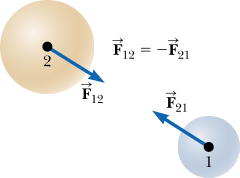
\includegraphics[scale=0.4]{terza_legge_newton}
\end{figure*}
\noindent Vediamo due corpi interagiscono che tra loro, la forza $\vec{F}_{12}$ esercitata dal corpo 1 sul corpo 2 è uguale in intensità ed è opposta
in verso alla forza $\vec{F}_{21}$ esercitata dal corpo 2 sul corpo 1:
\begin{equation*}
    \vec{F}_{12} = -\vec{F}_{21}
\end{equation*}

\paragraph{Diagramma di corpo libero}  Quando analizziamo un corpo soggetto a più forze, siamo interessati alla \textbf{forza risultante} 
su questo singolo corpo, che schematizzeremo come \emph{punto materiale}. Il diagramma di corpo libero, quindi, ci aiuta ad isolare solamente le forze che 
agiscono sul corpo ed eliminare dalla nostra analisi tutte le altre forze.

Nel \textbf{diagramma di corpo libero} è utilizzato il modello punto materiale per rappresentare il corpo come un punto e le forze che agiscono sul corpo sono applicate al punto.

\begin{figure*}[h]
    \centering
    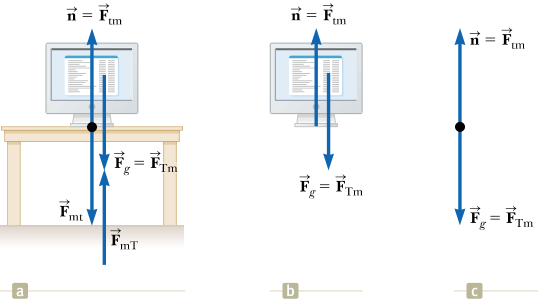
\includegraphics[scale=0.4]{diagramma_corpo_libero}
    \caption*{\small Il punto C dello schema rappresenta il \emph{diagramma di corpo libero}}
\end{figure*}

\section{Modelli di analisi}
\subsection{Punto materiale in equilibrio}
Se l’accelerazione di un corpo schematizzato come un punto materiale è nulla, il corpo verrà descritto con il modello \textbf{punto materiale in equilibrio}.
In questo schema, la forza risultante sul corpo è zero:
\begin{equation*}
    \sum \vec{F} = 0
\end{equation*}
\underline{Attenzione}: Anche un corpo che si muove a velocità costante può essere considerato \emph{in equilibrio}.

~\newline
\underline{Esempio: }
\begin{figure*}[h]
    \centering
    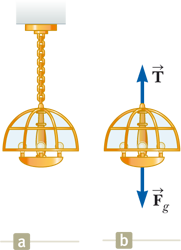
\includegraphics[scale=1]{lampada_in_equilibrio}
\end{figure*}
Le forze agenti sulla lampada sono la forza di gravità $\vec{F}_g$ verticale verso il basso e la forza di trazione $\vec{T}$ esercitata dalla catena verticalmente verso l'alto:
\begin{equation*}
    \sum F_y = 0 \;\; \rightarrow \;\; \sum F_y = T - F_g = 0 \;\; \rightarrow \;\; T = F_g
\end{equation*}
Si noti che, di nuovo, $\vec{T}$ e $\vec{F}_g$ \emph{non sono una coppia di forze di azione e reazione} perché esse sono applicate sullo stesso corpo, il lampadario.
La forza di reazione a $\vec{T}$  è applicata verso il basso dalla lampada alla catena.

\newpage
\subsection{Piano inclinato}
Esempio pratico:

\noindent Un’automobile di massa $m$ sta scivolando lungo una discesa ghiacciata inclinata di un angolo $\theta$, come mostrato in figura
\begin{figure*}[h]
    \centering
    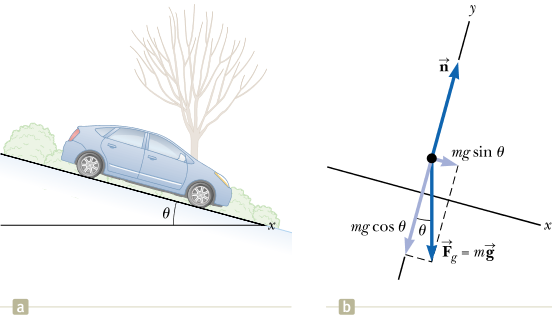
\includegraphics[scale=0.45]{piano_inclinato} ~~
    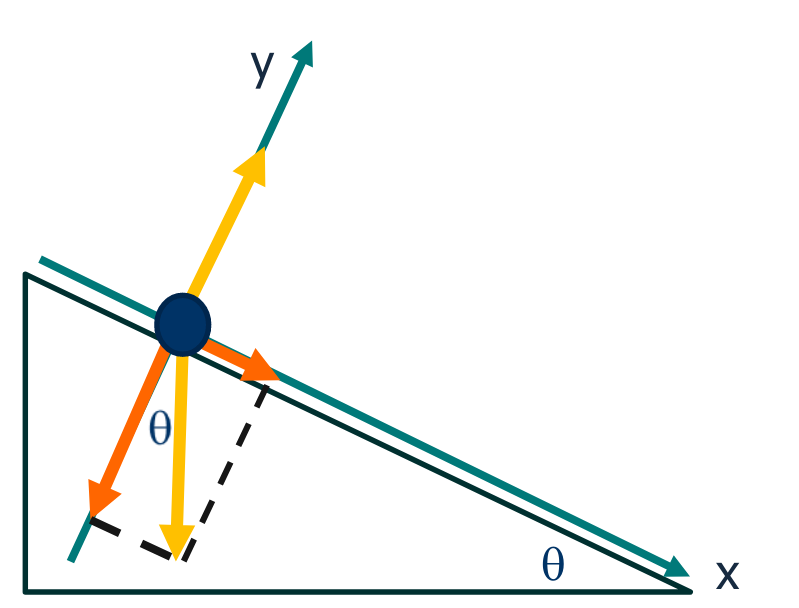
\includegraphics[scale=0.2]{piano_inclinato_forze}
\end{figure*}

\noindent Le forze in gioco sono:
\begin{itemize}
    \item \textbf{Forza peso} $\vec{F}_g = m\vec{g}$, sempre verticale verso il basso, divisa nelle sue componenti $x$ e $y$
    \begin{itemize}
        \item $\vec{F}_{gx} = mg \sin{\theta} = ma_x = \sum F_x$
        \item $\vec{F}_{gy} = mg \cos{\theta}$
    \end{itemize}
    \item \textbf{Reazione vincolare} $\vec{n}$, perpenticolare al piano
\end{itemize}
Sull'asse y non è presente accelerazione: $\sum F_y = n - mg \cos{\theta} = 0$ \newline
L'accelerazione in x quindi vale $a_x = g \sin{\theta}$ \newline
La reazione vincolare è pari a $n = mg \cos{\theta}$

\section{Forze di attrito}
Quando un corpo è in moto o su di una superficie o in un mezzo viscoso, come l’aria o l’acqua, 
nasce una \emph{resistenza al moto} a causa delle interazioni tra il corpo ed il mezzo che lo circonda. Questa resistenza prende il nome di \textbf{forza di attrito}.
\begin{figure*}[h]
    \centering
    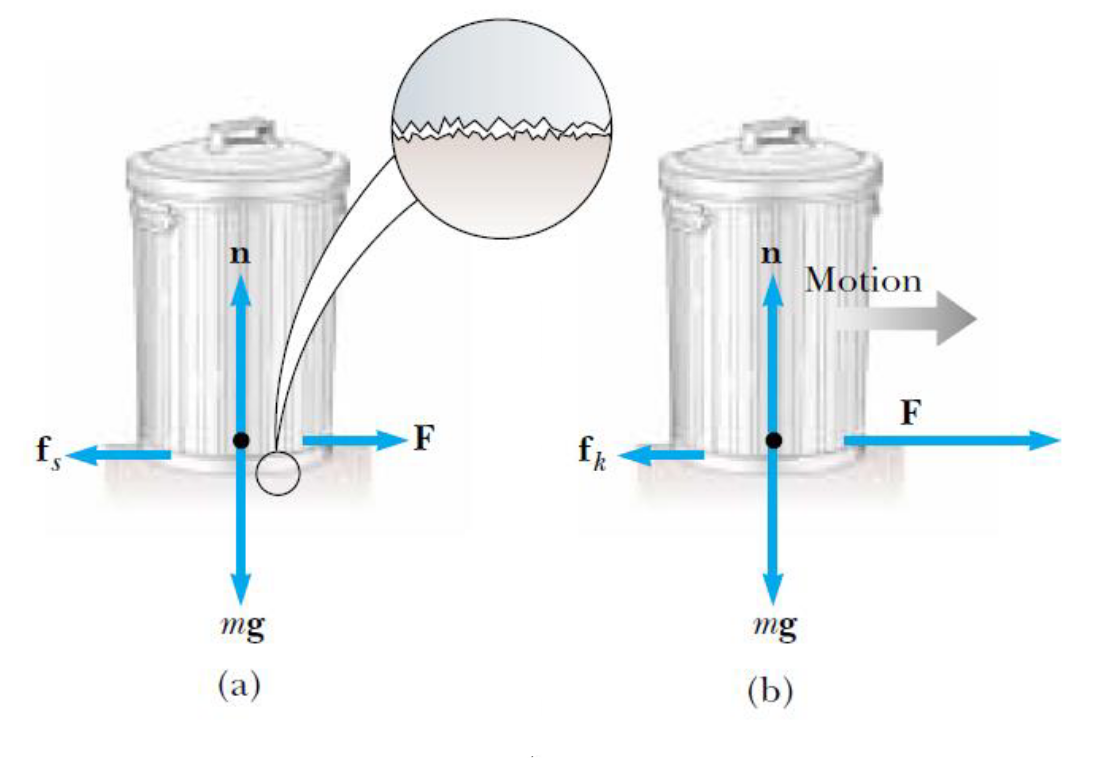
\includegraphics[scale=0.23]{attrito_bidone}
\end{figure*}

\paragraph{Attrito statico}
Se applichiamo a un'oggetto una forza $\vec{F}$ esterna orizzontale verso destra e se la forza $\vec{F}$ che applichiamo è piccola, l'oggetto rimarrà fermo.

La forza che agisce sull'oggetto e che contrasta $\vec{F}$ impedendogli di muoversi verso sinistra, prende il nome di forza di \textbf{attrito statico} $\vec{f}_s$.

Fino a quando l'oggetto rimane fermo, si ha $\vec{f}_s = \vec{F}$. Quindi se $\vec{F}$ aumenta, aumenterà anche $\vec{f}_s$. In ugual modo, se $\vec{F}$ diminuisce, diminuirà anche $\vec{f}_s$ .

L’intensità della forza di attrito statico tra due superfici qualunque a contatto tra loro può assumere i valori
\begin{equation*}
    f_s \le \mu_s n
\end{equation*}
dove la costante adimensionale $\mu_s$ è chiamata \textbf{coefficiente di attrito statico}.

\paragraph{Attrito dinamico}
Aumentando il valore di $\vec{F}$, l'oggetto arriverà sul punto di iniziare a muoversi, $\vec{f}_s$ raggiunge il suo valore massimo, $\vec{f}_{s,max}$.

Quando F supera il valore $\vec{f}_{s,max}$, il bidone inizierà a muoversi e, quindi, ad accelerare verso destra. La forza di attrito su di un corpo in movimento prende il nome di \textbf{forza di attrito dinamico} $\vec{f}_k$.
La forza risultante è $\vec{F} - \vec{f}_k > 0$ (moto).

Quando il bidone è in moto, il valore della forza di attrito dinamico che agisce sul corpo è \underline{minore} di $\vec{f}_{s,max}$. 

L’intensità della forza di attrito dinamico tra due superfici qualunque a contatto tra loro è
\begin{equation*}
    f_k = \mu_k n
\end{equation*}
dove la costante adimensionale $\mu_k$ è chiamata \textbf{coefficiente di attrito dinamico}.

\begin{figure*}[h]
    \centering
    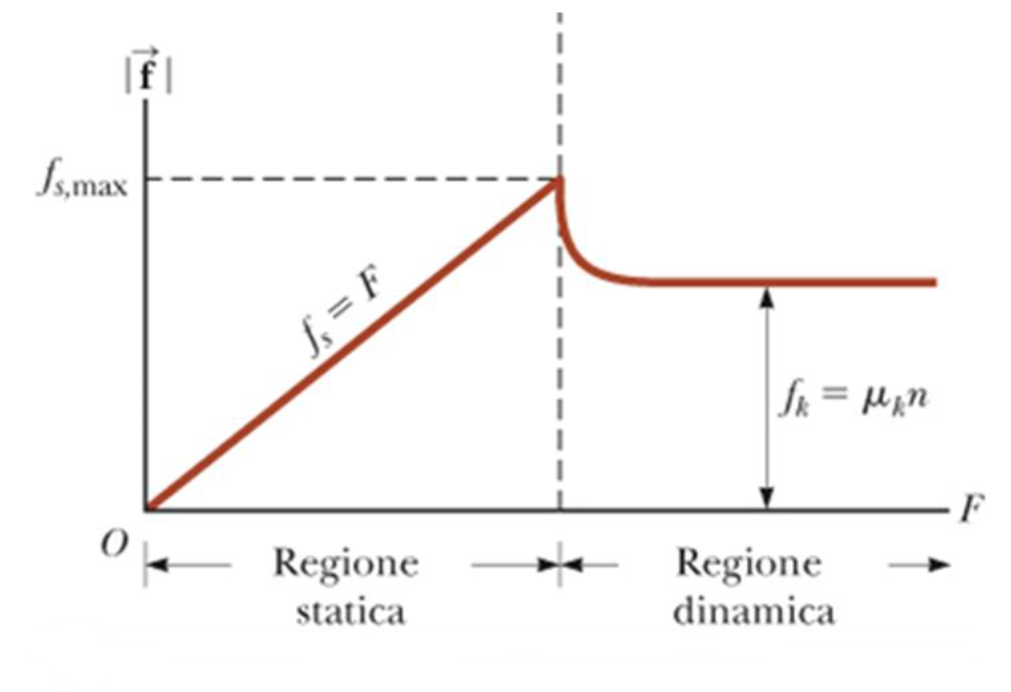
\includegraphics[scale=0.3]{forze_attrito_grafico}
\end{figure*}
\noindent Sperimentalmente, sia $\vec{f}_k$ che $\vec{f}_{s,max}$ hanno moduli proporzionali al modulo di $n$.

\newpage
\section{Altre applicazioni delle leggi di Newton}

\subsection{Estensione del Moto Circolare Uniforme}
Nel moto circolare uniforme il punto materiale si muove con velocità in modulo $v$ costante lungo una traiettoria circolare di raggio $r$.
Il punto materiale si muove con \textbf{accelerazione centripeta} di modulo
\begin{equation*}
    a_c = \frac{v^2}{r}
\end{equation*}
L'accelerazione è diretta verso il \emph{centro} ed è perpendicolare a $v$. Per la seconda legge di Newton, la forza risultante che produce l'accelerazione centripeta
può essere messa in relazione con l'accelerazione come segue:
\begin{equation*}
    \sum F = ma_c = m \frac{v^2}{r}
\end{equation*}
Una forza che produce un’accelerazione centripeta deve agire nella direzione che punta al \textbf{centro} del percorso circolare e provoca una variazione della direzione del vettore velocità.

\subsection{Moto Circolare non Uniforme}
se un punto materiale si muove con velocità di modulo variabile su un percorso circolare, ci deve essere, oltre alla componente radiale della accelerazione, una componente tangenziale di modulo $\abs{\tfrac{dv}{dt}}$. Quindi, anche la forza agente sulla particella deve avere una componente tangenziale ed una radiale.
\begin{figure*}[h]
    \centering
    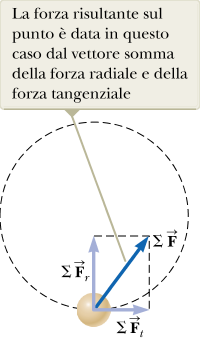
\includegraphics[scale=0.4]{newton_moto_circolare_non_uniforme.png}
\end{figure*}

\noindent L'accelerazione risultante è:
\begin{equation*}
    \vec{a} = \vec{a_r} + \vec{a_t}
\end{equation*}
E di conseguenza la forza risultante esercitata sulla particella è:
\begin{equation*}
    \sum \vec{F} = \sum \vec{F_r} + \sum \vec{F_t}
\end{equation*}
Il vettore $\sum \vec{F_r}$ è diretto verso il centro della circonferenza ed è responsabile dell’accelerazione centripeta. 
Il vettore $\sum \vec{F_t}$ tangente alla circonferenza è responsabile della accelerazione tangenziale, che rappresenta una variazione nel tempo del modulo 
della velocità del punto materiale.

\section{Moto in presenza di forze frenanti}
Consideriamo ora l'interazione tra il corpo in movimento e il mezzo nel quale esso si muove, che può essere un liquido o un gas. Il mezzo esercita una \textbf{forza frenante} $\vec{R}$ sul corpo che lo sta attraversando.
L’intensità di $\vec{R}$ dipende dal \emph{modulo} della velocità del corpo, mentre il verso di $\vec{R}$ è sempre \emph{opposto alla direzione di moto} del corpo relativamente al mezzo attraversato.

\subsection{Forza frenante proporzionale alla velocità del corpo}
Se facciamo l’ipotesi che la forza frenante che agisce su un corpo in moto in un liquido o in un gas sia proporzionale alla velocità del corpo, allora la forza frenante può essere espressa come
\begin{equation*}
    R = -b\vec{v}
\end{equation*}
dove $b$ è una \textbf{costante} il cui valore dipende dalle \emph{proprietà del mezzo}, dalla forma e dalle dimensioni del corpo, e $\vec{v}$ è la velocità del corpo rispetto al mezzo.

~\newline
\underline{Esempio}: Sfera di massa $m$ lasciata cadere in un liquido.
\begin{figure*}[h]
    \centering
    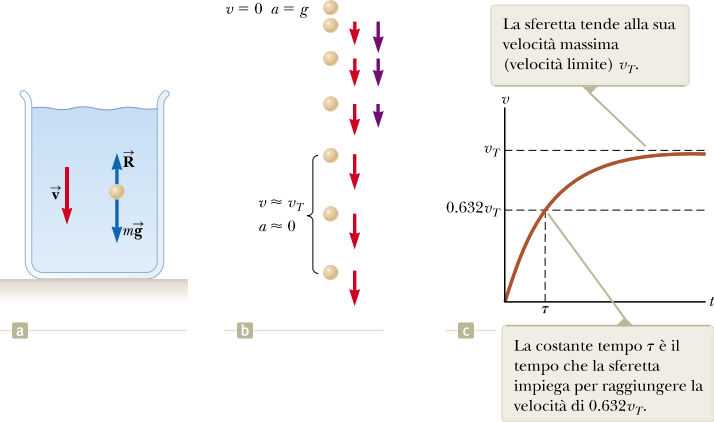
\includegraphics[scale=0.4]{sfera_fluido.png}
\end{figure*}

\noindent La sommatoria delle forze che agiscono è 
\begin{equation*}
    \sum F_y = mg - bv = ma
\end{equation*}
Al crescere del tempo cresce la velocità e di conseguenza cresce anche l'intensità della forza frenante R. Si arriverà ad un punto in cui $\abs{R} = \abs{F_p}$
In queste condizioni l'accelerazione diventerà nulla $a=0$ e la velocità tenderà alla \textbf{velocità limite} $v_T$.
\begin{align*}
    mg - bv_T = 0 \;\; \rightarrow \;\; v_T = \frac{mg}{b}
\end{align*}

~\newline
La velocità in funzione del tempo si ricava con:
\begin{equation*}
    v = v_T(1-e^{-t/\tau})
\end{equation*}
dove la \textbf{costante di tempo} $\tau = \tfrac{m}{b}$ corrisponde all’intervallo di tempo nel quale la sferetta partendo da ferma raggiunge il $63.2\%$ del valore della sua $v_T$.

\chapter{Energia}

\section{Energia di un sistema}
\subsection{Lavoro compiuto da una forza costante}
In fisica, il \textbf{lavoro} è l'\emph{\underline{energia} scambiata tra due sistemi} quando avviene uno spostamento attraverso l'\emph{azione di una forza}, o una risultante di forze, che ha una componente non nulla nella direzione dello spostamento. 
Pertanto, ha le dimensioni di una forza applicata lungo una determinata distanza. 

Il lavoro W compiuto su un sistema da un agente che esercita su di esso una forza costante è uguale al prodotto tra il \textbf{modulo $F$ della forza}, 
il \textbf{modulo $\Delta r$ dello spostamento} del punto di applicazione della forza e {\boldmath$\cos{\theta}$}, dove $\theta$ è l’angolo tra il vettore forza e il vettore spostamento:
\begin{equation*}
    W \equiv F \Delta r \cos{\theta}
\end{equation*}
L'unità di misura del \textbf{lavoro} è: $N \cdot m = kg \cdot m^2/s^2 = J \; \text{(joule)}$.

~\newline \underline{Alcune osservazioni}:
\begin{itemize}
    \item Una forza compie un lavoro nullo su un corpo se esso non viene spostato. Infatti, se $\Delta r$ = 0, l’Equazione fornisce $W$ = 0.
    \item Il lavoro compiuto da una forza su un corpo in movimento è zero quando la forza applicata è perpendicolare allo spostamento del suo punto di applicazione. Infatti, se $\theta = 90^\circ$ allora $W = 0$ poiché $\cos{90^\circ} = 0$.
    \item Il lavoro compiuto dalla forza applicata su un sistema è positivo quando la proiezione di $\vec{F}$ lungo la direzione di $\Delta \vec{r}$ ha lo stesso verso dello spostamento.
    Quando la proiezione di $\vec{F}$ lungo la direzione di $\Delta \vec{r}$ ha verso opposto a quello dello spostamento, $W$ è negativo.
    \item Una considerazione importante nell’approccio ai problemi consiste nel pensare al lavoro come \textbf{trasferimento di energia}. Se $W$ è il lavoro compiuto su un sistema 
    e $W$ è positivo, dell’energia viene trasferita \emph{al sistema}; se $W$ è negativo, dell’energia è trasferita \emph{dal sistema}.
\end{itemize}

\subsection{Prodotto scalare tra due vettori}
Per tener conto del modo in cui i vettori forza e spostamento sono combinati, è utile introdurre un appropriato strumento matematico chiamato \textbf{prodotto scalare tra due vettori}. 
Il prodotto scalare tra i vettori $\vec{A}$ e $\vec{B}$ viene indicato con l’espressione $\vec{A}\cdot\vec{B}$.

Il prodotto scalare tra due vettori $\vec{A}$ e $\vec{B}$ è una quantità scalare uguale al prodotto dei moduli dei due vettori per il coseno dell’angolo $\theta$ compreso tra di essi:
\begin{equation*}
    \vec{A} \cdot \vec{B} = AB\cos{\theta}
\end{equation*}
Confrontando tale definizione con l'equazione , possiamo esprimere l’equazione del \textbf{lavoro} sotto forma di un prodotto scalare:
\begin{equation*}
    W = F \cdot \Delta r \cdot \cos{\theta} = \vec{F} \cdot \Delta \vec{r}
\end{equation*}

\section{Lavoro di una forza variabile}
Consideriamo un punto materiale che si sposta lungo l’asse x sotto l’azione di una \emph{forza che varia con la posizione}. In tale situazione, non è possibile utilizzare l'equazione vista in
precedenza per calcolare il lavoro fatto dalla forza in quanto tale relazione si applica solo se il vettore $\vec{F}$ rimane costante in modulo, direzione e verso.

\begin{wrapfigure}{r}{0.20\textwidth}
    \centering
    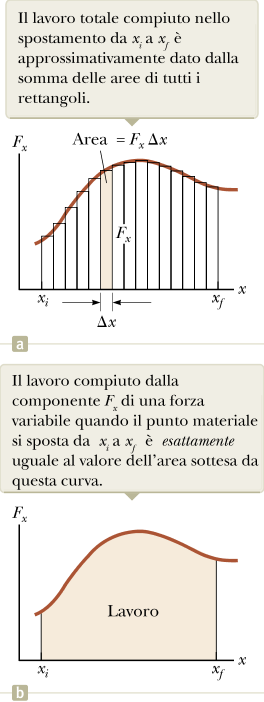
\includegraphics[width=0.20\textwidth]{lavoro_forza_variabile.png}
\end{wrapfigure}
Possiamo suddividere l'intervallo in tanti piccoli intervalli di spostamento $\Delta x$ e assumere che la forza in ogni intervallo valga un dato $F_x$. 
Il lavoro complessivo sarà quindi approssimato con la sommatoria
del lavoro di ogni intervallo:
\begin{equation*}
    W \approx \sum_{x_i}^{x_f} F_x \Delta x
\end{equation*}
Per migliorare questa approssimazione valutiamo il limite per $\Delta x$ che tende a 0:
\begin{align*}
    \lim_{\Delta x \to 0} \sum_{x_i}^{x_f} F_x \Delta x &= \int_{x_i}^{x_f} F_x \; dx & W&= \int_{x_i}^{x_f} F_x \; dx
\end{align*}
Se sul corpo agiscono più forze (nella direzione x):
\begin{equation*}
    \sum W = W_{est} = \int_{x_i}^{x_f} \big(\sum F_x \big) \; dx
\end{equation*}
Se una forza risultante variabile in modulo e direzione agisce sul corpo:
\begin{equation*}
    \sum W = W_{est} = \int_{x_i}^{x_f} \big(\sum \vec{F} \big) \cdot d \; \vec{r}
\end{equation*}


\subsection{Lavoro compiuto da una molla}
Lo schema di un sistema fisico molto comune nel quale la forza varia in funzione della posizione è mostrato in Figura. Il sistema è un blocco che giace su una superficie orizzontale senza attrito, collegato ad una molla.
Se la molla viene allungata o compressa di un piccolo tratto rispetto alla sua lunghezza di riposo (equilibrio), essa esercita sul blocco una forza che matematicamente può essere espressa nella forma
\begin{align*}
    F_s &= -kx & &\text{\textbf{Legge di Hooke}} 
\end{align*}
dove $x$ indica la posizione del blocco rispetto alla sua posizione di equilibrio $(x = 0)$ e $k$ è una costante positiva chiamata \textbf{costante elastica} della molla.

\newpage
\begin{figure*}[h]
    \centering
    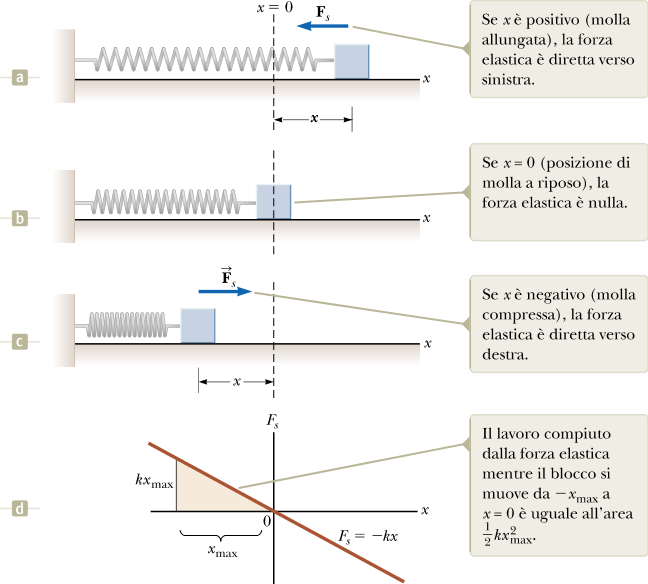
\includegraphics[scale=0.4]{lavoro_molla.png}
\end{figure*}
Il valore di k dà una misura della rigidità della molla. Molle “rigide” hanno grandi valori di k, mentre per molle “morbide” i valori di k sono piccoli. L'unità di misura di $k$ corrisponde a $N/m$.
Il lavoro della forza elastica sarà
\begin{equation*}
    W_s = \int_{x_i}^{x_f}F_s \;dx
\end{equation*}
Ipotizzando di partire dal punto di massima compressione della molla ($-x_{max}$) ed arrivare al punto $x=0$
\begin{equation*}
    W_s = \int_{x_i}^{x_f}F_s \; dx = \int_{-x_{max}}^{0} (-kx) \; dx = \tfrac{1}{2}kx^2_{max}
\end{equation*}
Per uno spostamento arbitrario da $x_i$ a $x_f$:
\begin{equation*}
    W_s = \int_{x_i}^{x_f}F_s \; dx = \tfrac{1}{2} kx_i^2 - \tfrac{1}{2}kx_f^2
\end{equation*}
Da notare che, per qualunque spostamento in cui punto iniziale e punto finale coincidono, il lavoro è nullo.

Consideriamo ora il lavoro compiuto sul blocco da un agente esterno che applica una forza sul blocco mentre questo si sposta molto lentamente da $xi = -x_{max}$ a $x_f = 0$.
Possiamo calcolare questo lavoro osservando che per ogni valore della posizione, la forza applicata $\vec{F}_{app}$ è uguale in modulo e opposta in verso alla forza elastica $\vec{F}_s$, cosicché
\begin{gather*}
    F_{app} = -(-kx) = kx \\ 
    W_{F_{app}} = \int_{0}^{x_{max}} F_{app} \; dx = \int_{0}^{x_{max}} kx \; dx = \tfrac{1}{2}kx^2_{max}
\end{gather*}
Per uno spostamento arbitrario del blocco, il lavoro compiuto sul sistema dall'agente esterno è dato da 
\begin{equation*}
    W_{F_{app}} = \int_{x_i}^{x_f} F_{app} \; dx = \int_{x_i}^{x_f} kx \; dx = \tfrac{1}{2}kx_f^2 - \tfrac{1}{2} kx_i^2
\end{equation*}

\section{Energia Cinetica}
Una possibile \emph{conseguenza del lavoro} compiuto su un sistema è la \emph{variazione della sua velocità}. L'\textbf{energia cinetica} è l'energia che un corpo possiede a causa del proprio movimento.

\begin{figure*}[h]
    \centering
    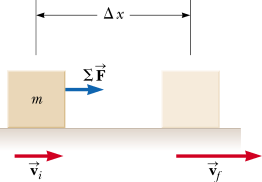
\includegraphics[scale=0.4]{energia_cinetica_schema.png}
\end{figure*}
La figura mostra un blocco di massa $m$ che si muove verso destra sotto l’azione di una forza risultante $\sum \vec{F}$ verso destra. Dalla seconda legge di Newton sappiamo che il blocco si muove con un’accelerazione $\vec{a}$.
Essendo la forza costante, il moto è \emph{uniformemente accelerato}. Per cui vale la relazione
\begin{gather*}
    v_f^2-v_i^2 = 2a(x_f-x_i) = 2\tfrac{F}{m}(x_f-x_i) \\
    F(x_f-x_i) = \tfrac{1}{2}m(v_f^2-v_i^2) = \tfrac{1}{2}mv_f^2 - \tfrac{1}{2}mv_i^2 = W
\end{gather*}
Definendo l'\textbf{energia cinetica} come
\begin{equation*}
    K \equiv \tfrac{1}{2}mv^2
\end{equation*}
notiamo quindi che il \textbf{lavoro} non è altro che \textbf{la variazione dell'energia cinetica}.
\underline{Teorema dell'energia cinetica}:
\begin{gather*}
    W = \tfrac{1}{2}mv_f^2 - \tfrac{1}{2}mv_i^2 = K_f - K_i = \Delta K \\
    W = \Delta K
\end{gather*}
L'unità di misura dell'energia cinetica è il \textbf{Joule}.

\section{Energia potenziale}
\subsection{Energia potenziale gravitazionale}
Pensiamo a un sistema costituito da un libro e dalla Terra, interagenti attraverso la forza gravitazionale.
Compiamo un certo lavoro sul sistema sollevando lentamente il libro che compie uno spostamento verticale $\Delta \vec{r} = (y_f - y_i)\hat{j}$.

\begin{figure*}[h]
    \centering
    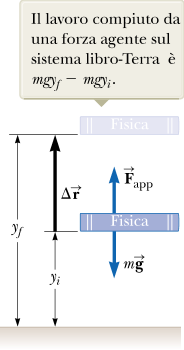
\includegraphics[scale=0.4]{energia_potenziale_schema.png}
\end{figure*}
Il lavoro compiuto sul sistema deve manifestarsi come un aumento di energia del sistema. Il libro è in quiete prima che compiamo il lavoro ed è in quiete dopo che lo abbiamo compiuto. Quindi, non c’è variazione dell’energia cinetica del sistema.

Possiamo dire che quando il libro si trova nella posizione più alta, l’energia del sistema ha la \emph{potenzialità di diventare energia cinetica}, che non si manifesta finché non lasciamo cadere il libro. Pertanto, il meccanismo di immagazzinamento di energia prima che il libro venga lasciato cadere è chiamato \textbf{energia potenziale}.

Il lavoro compiuto dall'agente esterno quando il corpo viene sollevato è
\begin{equation*}
    W_{est} = (\vec{F}_{app})\cdot \Delta \vec{r} = (mg\hat{j})\cdot[(y_f-y_i)\hat{j}] = mgy_f-mgy_i
\end{equation*}
Pertanto possiamo identificare la quantità $mgy$ come l’energia potenziale gravitazionale $U_g$ di un sistema di un corpo di massa $m$ e della Terra:
\begin{equation*}
    U_g \equiv mgy
\end{equation*}
L’energia potenziale gravitazionale si misura in \textbf{Joule}, cioè nelle stesse unità del lavoro e dell’energia cinetica.

L'equazione del lavoro può essere riscritta come
\begin{equation*}
    W_{est} = \Delta U_g
\end{equation*}
che matematicamente dice che il lavoro esterno compiuto sul sistema in questa situazione si manifesta come \emph{variazione dell’energia potenziale gravitazionale} del sistema.

L’\textbf{energia potenziale gravitazionale} \textbf{dipende unicamente dall’}\textbf{altezza del corpo} rispetto alla superficie della Terra. Supponendo infatti che lo spostamento $\Delta \vec{r}$
abbia una componente $x$ e una componente $y$ vediamo che 
\begin{align*}
    W_{est} &= (\vec{F}_{app})\cdot \Delta \vec{r} \\
    &= mg\hat{j} \cdot (\Delta x \hat{i} + \Delta y \hat{j}) = mg\Delta y \\ 
    &= mgy_f - mgy_i
\end{align*}

\subsection{Energia potenziale elastica}
Consideriamo un sistema costituito da un blocco e da una molla. La forza che la molla esercita sul blocco è data da $F_s = -kx$.
Il lavoro esterno compiuto da una forza applicata $F_{app}=-(-kx)$ su un sistema formato da blocco-molla è dato dall'equazione
\begin{equation*}
    W_{F_{app}} = \tfrac{1}{2} kx_f^2 -\tfrac{1}{2} kx_i^2
\end{equation*}
Vediamo che il lavoro compiuto sul sistema è uguale alla differenza tra i valori iniziale e finale di una espressione che dipende dalla configurazione del sistema.
La funzione \textbf{energia potenziale elastica} associata al sistema blocco–molla è definita da:
\begin{equation*}
    U_s \equiv  \tfrac{1}{2}kx^2
\end{equation*}
L'equazione del lavoro può quindi essere espressa come
\begin{equation*}
    W_{F_{app}} = \Delta U_s
\end{equation*}


\section{Forze conservative e non conservative}

\subsection{Forze conservative}
Le \textbf{forze conservative} godono delle due seguenti proprietà, tra loro equivalenti:
\begin{enumerate}
    \item Il lavoro compiuto da una forza conservativa agente su un punto materiale che si muove tra due punti qualsiasi \emph{non dipende dal percorso}.
    \item Il lavoro compiuto da una forza conservativa agente su un punto materiale che descrive un qualsiasi percorso chiuso è nullo. (Un percorso chiuso è una linea in cui il punto di partenza e il punto di arrivo coincidono.)
\end{enumerate}
Sono forze conservative, ad esempio, la \emph{forza di gravità} (forza peso) e la \emph{forza elastica}. Infatti il lavoro compiuto da queste forze dipende solamente dalla \emph{posizione iniziale} e dalla \emph{posizione finale}, 
non dal percorso che ha seguito il corpo.

In generale, il lavoro $W_{int}$ compiuto da una forza conservativa su un elemento di un sistema quando questo si sposta da un punto ad un altro è uguale alla differenza tra l’energia potenziale del sistema iniziale e quella finale:
\begin{equation*}
    W_{int} = U_i - U_f = -\Delta U
\end{equation*}

\subsection{Forze non conservative}
Una forza è non conservativa se \emph{non soddisfa} le proprietà 1 e 2 valide per le forze conservative. Il lavoro compiuto da una forza non conservativa, \emph{dipende dal percorso fatto}. 

\subsection{Relazione tra forze conservative ed energia potenziale}
Immaginiamo un sistema di punti materiali nel quale una forza conservativa $\vec{F}$ agisce fra le singole particelle e che la configurazione di tale sistema varia a causa del moto di un punto lungo l’asse $x$. 
Quindi, possiamo calcolare il lavoro interno compiuto da questa forza mentre il punto si muove lungo l’asse $x$
\begin{equation*}
    W_{int} = \int_{x_i}^{x_f} = F_x \; dx = -\Delta U
\end{equation*}
che possiamo anche esprimere nella forma
\begin{equation*}
    \Delta U = U_f - U_i = -\int_{x_i}^{x_f} F_x \; dx
\end{equation*}
Pertanto è possibile esprimere la \textbf{funzione energia potenziale} come
\begin{equation*}
    U_f = -\int_{x_i}^{x_f} F_x \; dx + U_i
\end{equation*}
stabilendo una posizione arbitraria di riferimento ($U_i$) e misurando la variazione di energia potenziale rispetto a tale posizione.

\section{Conservazione dell'energia}
Esistono dei meccanismi di accumulo dell'energia e meccanismi di trasmissione di energia.
Le forme di accumulo dell'energia sono:
\begin{itemize}
    \item \textbf{Energia cinetica} ($K$), legata al movimento dei costituenti di un sistema
    \item \textbf{Energia potenziale} ($U$), legata alla configurazione del sistema
    \item \textbf{Energia interna} ($E_{int}$), legata alla temperatura
\end{itemize}
I meccanismi di trasferimento dell'energia sono:
\begin{itemize}
    \item \textbf{Lavoro meccanico} ($W$)
    \item \textbf{Onde meccaniche} ($T_{OM}$)
    \item \textbf{Calore} ($Q$)
    \item \textbf{Trasferimento di materia} ($T_M$)
    \item \textbf{Trasmissione elettrica} ($T_E$)
    \item \textbf{Radiazioni elettromagnetiche}  ($T_{EM}$)
\end{itemize}

L'aspetto centrale della nostra discussione è che l’energia non può essere né creata, né distrutta: l’energia si \emph{conserva} sempre.
Quindi se l’energia totale di un sistema subisce una variazione, è necessario che una quantità di energia uguale alla variazione abbia attraversato i confini del sistema, con un meccanismo di trasferimento simile a quelli sopra elencati.

L’enunciato più generale del \textbf{principio di conservazione dell’energia} è contenuto nella equazione della conservazione dell’energia:
\begin{equation*}
    \Delta E_{sistema} = \sum T
\end{equation*}
in cui Esistema è l’energia totale del sistema, che comprende tutte le forme di immagazzinamento dell’energia e T (sta per trasferimento) è la quantità di energia 
trasferita mediante vari meccanismi attraverso la superficie che delimita il sistema.

\underline{Attenzione}: in un \textbf{sistema isolato} non c'è scambio di energia, $\Delta E_{sistema} = 0$.

~\newline È possibile estendere l'equazione della conservazione dell'energia in una forma più estesa:
\begin{equation*}
    \Delta K + \Delta U + \Delta E_{int} = W + Q + T_{OM} + T_{M} + T_{E}+ T_{EM}
\end{equation*}
che è la rappresentazione matematica fondamentale, in versione energia, del modello di analisi \textbf{sistema non isolato}.
Se si verifica il caso in cui tutti i termini a secondo membro si annullano, parleremo di sistema isolato.  

\subsection{Energia meccanica e conservazione dell'energia meccanica}
Supponiamo di aver sollevato un corpo fino a $y_i$ e calcoliamo il lavoro compiuto dalla forza peso nella caduta (da $y_i$ a $y_f$)
\begin{align*}
    W_g &= -mg\hat{j} \cdot (y_f - y_i) \hat{j} = mgy_i - mgy_f \\ &=U_i - U_f = -\Delta U
\end{align*}
Per il teorema del lavoro e dell'energia cinetica sappiamo che 
\begin{equation*}
    W_g = K_f - K_i = \Delta K
\end{equation*}
Mettendo in relazione le due equazioni:
\begin{align*}
    \Delta K &= -\Delta U \\
    K_f - K_i &= U_i - U_f \\
    K_f + U_f &= K_i + U_i \\
    E_{mecc_f} &= E_{mecc_i}
\end{align*}
Definiamo quindi l'\textbf{energia meccanica} come:
\begin{equation*}
    E_{mecc} = K + U
\end{equation*}
Ci si rende subito conto che durante il processo di caduta, in ogni momento, \textbf{l'energia meccanica} rimane la stessa, ovvero si \textbf{conserva}.
Il risultato si può applicare a tutti i sistemi isolati in cui siano coinvolte solo Forze Conservative.

\subsection{Sistemi con attrito dinamico}
Lo spostamento che appare nell’espressione del lavoro è lo spostamento del \emph{punto di applicazione della forza}.
Nella realtà la forza di attrito è distribuita su tutta l’area di contatto del corpo che scivola sulla superficie e non può certo essere localizzata in un punto.
Il valore delle forze di attrito nei vari punti di contatto cambia continuamente al cambiare delle saldature generate durante il contatto delle due superfici. 

Di fatto lo spostamento del punto di applicazione della forza di attrito non può essere calcolato e, di conseguenza, nemmeno il lavoro della forza di attrito.

Il teorema lavoro-energia cinetica è valido nel caso di una particella puntiforme o di un corpo che possa essere schematizzato come un punto materiale. Però, in presenza di forze di attrito, il lavoro di queste forze non può essere calcolato. In questa situazione la seconda equazione di Newton rimane ancora valida, mentre il teorema lavoro-energia cinetica non è più utilizzabile.

Supponiamo che su un corpo agiscano più forze, compreso l'attrito. La risultante di queste forze rimane costante. Partiamo dalla seconda legge di Newton
\begin{align*}
    \left(\sum \vec{F}_x \right) &= ma_x \\
    \left(\sum \vec{F}_x \right) \Delta x &= (ma_x) \Delta x
\end{align*}
Se la risultante rimane costante, allora il corpo è in moto rettilineo uniformemente accelerato:
\begin{align*}
    a_x &= \frac{v_f - v_i}{t} & \Delta x &= \tfrac{1}{2}(v_i + v_f)t
\end{align*}
\begin{align*}
    \left(\sum \vec{F}_x \right) \Delta x &= m \left(\frac{v_f - v_i}{t} \right)\tfrac{1}{2}(v_i+v_f)t \\
    \left(\sum \vec{F}_x \right) \Delta x &= \tfrac{1}{2}mv_f^2 - \tfrac{1}{2} mv_i^2
\end{align*}
Se la risultante è costituita solamente dalla forza d'attrito:
\begin{equation*}
    \left(\sum \vec{F}_x \right) \Delta x = -f_k \Delta x = \tfrac{1}{2}mv_f^2 - \tfrac{1}{2} mv_i^2 = \Delta K
\end{equation*}

Consideriamo ora un sistema isolato composto da un libro con una velocità iniziale $v_i>0$ che scorre su un tavolo. L'unica forza che agisce sul libro è la forza di attrito.
L'energia del sistema è data da:
\begin{equation*}
    E_{system} = \Delta K + \Delta E_{int} = 0
\end{equation*}
Conoscendo già la variazione dell'energia cinetica del libro:
\begin{align*}
    -f_kd + \Delta E_{int} = 0 \\
    \Delta E_{int} = f_kd
\end{align*}
Vediamo quindi che la forza d'attrito \emph{trasforma} l'energia cinetica in energia interna. L'aumento dell'energia interna del sistema è uguale al prodotto della forza d'attrito
per la distanza totale percorsa dal corpo.

\subsection{Generalizzazione della legge di conservazione dell'energia}
Supponiamo di avere un \textbf{sistema isolato} in cui possa cambiare sia l'\emph{energia cinetica} che l'\emph{energia potenziale}.
Essendo il sistema isolato, non c'è variazione di energia:
\begin{gather*}
    \Delta E_{system} = 0 \\
    \Delta U + \Delta K + \Delta E_{int} = 0 \\
    \Delta U + \Delta K = -\Delta E_{int}
\end{gather*}
Conosciamo già il valore della variazione di energia interna: $\Delta E_{int} = f_k d$
\begin{gather*}
    \Delta U + \Delta K = -f_k d\\ 
    \Delta E_{mecc} = -f_k d
\end{gather*}
Vediamo quindi che la quantità di energia meccanica ($\Delta E_{mecc} = \Delta U + \Delta K$) persa è dovuta al lavoro della forza d'attrito.

\section{Potenza}
La potenza è definita come l'energia trasferita per unità di tempo. L’energia trasferita nell’unità di tempo è detta \textbf{potenza istantanea P} ed è definita come:
\begin{equation*}
    P \equiv \frac{dE}{dt}
\end{equation*}
Se una forza esterna è applicata ad un corpo ed il lavoro compiuto sul corpo da questa forza in un intervallo di tempo $\Delta t$ è $W$, la \textbf{potenza media} in quell'intervallo 
di tempo è
\begin{equation*}
    P_{media} \equiv \frac{W}{\Delta t}
\end{equation*}
In modo analogo a quanto già fatto per definire velocità e accelerazione in un istante di tempo, possiamo definire la potenza istantanea come il valore limite della potenza media, al tendere a zero di $\Delta t$:
\begin{equation*}
    P = \lim_{\Delta t \to 0} \frac{W}{\Delta t} = \frac{dW}{dt}
\end{equation*}
L'unità di misura della Potenza è il Watt: $1W = 1J/s = 1kg \cdot m^2/s^3$

\chapter{Quantità di moto e urti}

\section{Quantità di moto (sistema isolato)}
Per introdurre questa nuova quantità, consideriamo un sistema isolato composto da due particelle di massa $m_1$ ed $m_2$ che si muovono, ad un certo istante, con velocità $\vec{v}_1$ e $\vec{v}_2$.

Se una forza dovuta alla particella 1 (per esempio, una forza gravitazionale) agisce sulla particella 2, ci deve quindi essere una seconda forza – uguale in modulo ma opposta in verso – che la particella 2 esercita sulla 1.
In altre parole, queste due forze formano una coppia \emph{azione-reazione} nel senso del \emph{terzo principio di Newton}, e risulta $\vec{F}_{21} = \vec{F}_{12}$. Ovvero possiamo riscrivere l'equazione come
\begin{equation*}
    \vec{F}_{21} + \vec{F}_{12} = 0
\end{equation*}
Nel caso di un sistema di punti materiali, questa equazione ci dice che la somma delle forze che agiscono su un sistema isolato è \emph{zero}. Possiamo riscrivere l'equazione sostituendo
la forza con la quantità $m\vec{a}$, ottenendo
\begin{gather*}
    m_1\vec{a}_1 + m_2\vec{a}_2 = 0 \\ 
    m_1 \frac{dv_1}{dt} + m_2 \frac{dv_2}{dt} = 0 \\
\end{gather*}
Se le masse $m_1$ ed $m_2$ sono costanti, le possiamo portare dentro l’operatore di derivazione
\begin{gather*}
    \frac{d(m_1v_1)}{dt} + \frac{d(m_2v_2)}{dt} = 0 \\ 
    \tfrac{d}{dt}(m_1v_1 + m_2v_2) = 0
\end{gather*}

\paragraph{Definizione} Chiamiamo \textbf{quantità di moto} la \textbf{grandezza vettoriale} $m\vec{v}$:
\begin{equation*}
    p \equiv m\vec{v}
\end{equation*}
L'unità di misura di questa grandezza è $kg \cdot m/s$

~\newline Se la derivata della somma $m_1v_1 + m_2v_2$ è uguale a \emph{zero}, significa che la somma deve rimanere costante.
Notiamo quindi che la quantità di moto $p = m\vec{v}$, dove $m$ è la massa e $\vec{v}$ la velocità di una particella, soddisfa una proprietà importante: la somma di tutte le quantità di moto per un sistema isolato \textbf{si conserva}.

Ogni qualvolta due o più particelle di un sistema fisico isolato interagiscono, la quantità di moto totale del sistema rimane costante:
\begin{equation*}
    p_{tot} = p_1 + p_2 + \dotsb + p_{n} = constant
\end{equation*}

\paragraph{Seconda legge di Newton} È possibile esprimere la seconda legge della Dinamica in termini della quantità di moto. 
La seconda legge di Newton ci dice che la forza risultante applicata a un corpo è data dalla sua massa per l'accelerazione.
\begin{equation*}
    \sum \vec{F} = ma = m \frac{dv}{dt}
\end{equation*}
Essendo la massa costante, la possiamo portare all'interno dell'operatore di derivazione:
\begin{equation*}
    \sum \vec{F} = \frac{d(m\vec{v})}{dt} = \frac{d\vec{p}}{dt}
\end{equation*}
Vediamo quindi che la variazione della quantità di moto di un corpo non è altro che la forza risultante che agisce sullo stesso.

\section{Quantità di moto (sistema non isolato)}
Da un punto di vista energetico, un sistema non è isolato se c’è un flusso di energia attraverso i confini del sistema. Per quanto riguarda la conservazione della quantità di moto, un sistema è non isolato se la risultante delle forze esterne agenti sul sistema in un dato intervallo di tempo non è nulla. 
In tale situazione, possiamo immaginare che della quantità di moto venga trasferita al sistema proprio dalla risultante delle forze esterne.

Per iniziare ad approfondire questo importante concetto, facciamo l’ipotesi che una risultante delle forze $\sum \vec{F}$ agisca su un punto materiale e che tale forza possa variare nel tempo in accordo con la seconda legge di Newton.
\begin{align*}
    \sum \vec{F} &= \tfrac{d\vec{p}}{dt} & d\vec{p} &= \sum\vec{F} \; dt
\end{align*}
Integrando questa espressione nell’intervallo di tempo in cui agisce la forza, si ottiene la variazione di quantità di moto del punto materiale.
Se la quantità di moto del punto materiale cambia da $\vec{p}_i$ all’istante $t_i$ a $\vec{p}_f$ all’istante $t_f$, l'integrazione dell'equazione dà:
\begin{equation*}
    \Delta \vec{p} = \vec{p}_f - \vec{p}_i = \int_{t_i}^{t_f} \sum \vec{F} \; dt
\end{equation*}

\paragraph{Impulso} La quantità a secondo membro di questa equazione è chiamata impulso della risultante $\sum \vec{F}$	agente sul punto materiale nell’intervallo di tempo $\Delta t$:
\begin{align*}
    \vec{I} &= \int_{t_i}^{t_f} \sum \vec{F} \; dt & \Delta \vec{p} &= \vec{I}
\end{align*}

\section{Urti in una dimensione}
\paragraph{Definizione} L'\textbf{urto} è il termine fisico con il quale si identifica la collisione di due corpi che si scontrano. 
Due corpi interagiscono scambiandosi forze molto intense per intervalli di tempo molto piccoli. Si parla quindi di \textbf{approssimazione impulsiva}, intendendo che le forze 
che agiscono in questi brevi intervalli di tempo siano molto più intense di tutte le forze esterne presenti, permettendoci di trascurarle.

Tenendo solamente conto delle forze interne, possiamo rifarci al modello di sistema isolato in cui la \textbf{quantità di moto si conserva}.

\subsection{Urti anelastici}
Un \textbf{urto anelastico} è un urto in cui le energie cinetiche totali del sistema prima e dopo l’urto sono diverse (anche se la quantità di moto del sistema è conservata).
Gli urti anelastici sono di \emph{due tipi}:
\begin{enumerate}
    \item \textbf{Urti perfettamente anelastici}: Quando due oggetti si urtano e rimangono uniti l’uno all’altro (es. meteorite che colpisce la terra)
    \item \textbf{Urti anelastici}: Quando gli oggetti che si urtano non rimangono uniti, ma si ha ugualmente dissipazione di energia cinetica (es. una palla di gomma colpisce una superficie dura)
\end{enumerate}


Consideriamo un caso di \textbf{urto perfettamente anelastico}. Due punti materiali di massa $m_1$ ed $m_2$ che si muovono con velocità iniziali $\vec{v}_{1i}$ e $\vec{v}_{1i}$ lungo una retta.
I due punti materiali si urtano centralmente, rimangono uniti e si muovono, dopo l’urto, con una velocità comune $\vec{v}_f$. 

\begin{figure}[h]
    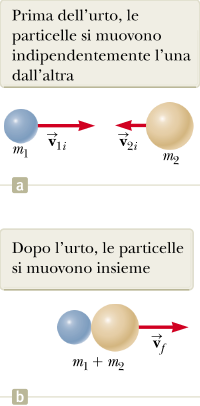
\includegraphics[scale=0.4]{urto_perfettamente_anelastico.png}
    \centering
\end{figure}
\noindent La quantità di moto rimane invariata prima e dopo l'urto:
\begin{equation*}
    \Delta \vec{p} = 0 \;\; \rightarrow \;\; \vec{p}_i = \vec{p}_f \;\; \rightarrow \;\; m_1\vec{v}_{1i} + m_2\vec{v}_{2i} = (m_1 + m_2) \vec{v}_f
\end{equation*}
La velocità finale quindi equivale a
\begin{equation*}
    \vec{v}_f = \frac{m_1\vec{v}_{1i} + m_2\vec{v}_{2i}}{m_1 + m_2}
\end{equation*}

\subsection{Urti elastici}
Un \textbf{urto elastico} tra due oggetti è un urto in cui l’energia cinetica totale del sistema è uguale prima e dopo l’urto (così come la quantità di moto totale).
Alcuni tipi di urti che avvengono nella realtà che quotidianamente ci circonda sono elastici solo \emph{approssimativamente}, esiste sempre una dissipazione di energia cinetica.

Gli unici urti che sono realmente elastici sono quelli che avvengono tra \emph{particelle subatomiche}. Tali urti possono essere descritti usando il modello sistema isolato sia per l’energia che per la quantità di moto. Infatti, in essi non vi è alcuna trasformazione di energia cinetica in altre forme di energia all’interno del sistema.

\begin{wrapfigure}{r}{0.25\textwidth}
    \centering
    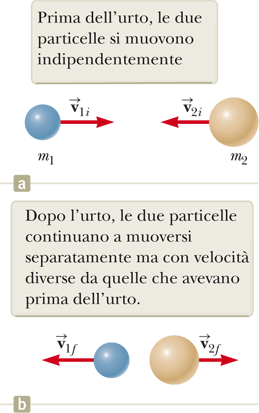
\includegraphics[width=0.25\textwidth]{urto_elastico.png}
\end{wrapfigure}
Consideriamo ora due punti materiali di massa $m_1$ ed $m_2$ che si muovono in linea retta con velocità iniziali date da $\vec{v}_{1i}$ e da $\vec{v}_{2i}$, come mostrato in figura

I due punti materiali urtano centralmente e dopo si allontanano dalla zona di interazione con velocità differenti, che indicheremo con $\vec{v}_{1f}$ e $\vec{v}_{2f}$.
Se la collisione è di tipo elastica, sia la quantità di moto che l'energia cinetica del sistema si devono conservare.
Quindi, assumendo che le velocità siano dirette lungo l’asse orizzontale abbiamo:
\begin{align*}
    \vec{p}_i = \vec{p}_f \;\; &\rightarrow \;\; m_1v_{1i} +  m_2v_{2i} = m_1v_{1f} +  m_2v_{2f} \\
    K_i = K_f \;\; &\rightarrow \;\;\tfrac{1}{2} m_1v_{1i}^2 + \tfrac{1}{2} m_2v_{2i}^2 = \tfrac{1}{2} m_1v_{1f}^2 + \tfrac{1}{2} m_2v_{2f}^2
\end{align*}
Riscriviamo l'equazione della conservazione dell'energia cinetica e scomponiamo i membri dell'equazione:
\begin{align*}
    m_1(v_{1i}^2 - v_{1f}^2) &= m_2(v_{2f}^2 - v_{2i}^2) \\
    m_1(v_{1i} - v_{1f})(v_{1i} + v_{1f}) &= m_2(v_{2f} - v_{2i})(v_{2f} + v_{2i})
\end{align*}
Separiamo ora i termini dell'equazione della conservazione della quantità di moto:
\begin{equation*}
    m_1(v_{1i} - v_{1f}) = m_2(v_{2f} - v_{2i})
\end{equation*}
Dividendo quindi l'equazione dell'energia cinetica per l'equazione della quantità di moto:
\begin{align*}
    v_{1i} + v_{1f} &= v_{2f} + v_{2i} \\ 
    v_{1i} - v_{2i} &= -(v_{1f} - v_{2f})
\end{align*}
Vediamo quindi che la velocità relativa prima dell'urto, $v_{1i} - v_{2i}$, è uguale e di segno opposto alla velocità relativa dopo l'urto, $-(v_{1f} - v_{2f})$.

Si supponga che le masse e le velocità iniziali delle due particelle siano note. Le precedenti equazioni possono essere risolte per calcolare le velocità finali in funzione delle velocità iniziali,
poiché si hanno due equazioni e due incognite. Il risultato è:
\begin{align*}
    v_{1f} &= \left( \frac{m_1 - m_2}{m_1 + m_2} \right) v_{1i} + \left( \frac{2m_2}{m_1 + m_2} \right) v_{2i} \\
    v_{2f} &= \left( \frac{2m_1}{m_1 + m_2} \right) v_{1i} + \left( \frac{m_2 - m_1}{m_1 + m_2} \right) v_{2i}
\end{align*}

\section{Centro di massa}
Descriveremo ora il moto complessivo di un sistema meccanico in termini del moto di un particolare punto, detto \textbf{centro di massa (CM)} del sistema.
Il sistema meccanico può essere costituito sia da un insieme di punti materiali, sia da un corpo continuo.

Vedremo che il centro di massa è un punto materiale che si muove come se tutta la massa del sistema fosse in esso concentrata. Il sistema si muove quindi come se la risultante delle forze esterne fosse applicata ad un singolo punto materiale posto nel centro di massa.

Si consideri ora un sistema composto da due particelle di massa $m_1$ e $m_2$ disposte lungo l'asse delle $x$.
\begin{figure}[h]
    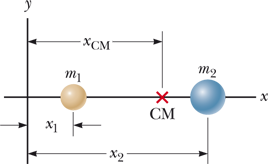
\includegraphics[scale=1]{centro_di_massa_asse_x.png}
    \centering
\end{figure}
Il \textbf{centro di massa} della coppia di punti materiali si troverà sempre sull'asse delle $x$ in un punto intermedio fra le due particelle. La sua coordinata è definita dalla relazione:
\begin{equation*}
    x_{CM} \equiv \frac{m_1x_1 + m_2x_2}{m_1 + m_2}
\end{equation*}

~\newline La definizione può essere estesa a $n$ punti materiali:
\begin{equation*}
    x_{CM} \equiv \frac{m_1x_1 + m_2x_2 + \cdots + m_nx_n}{m_1 + m_2 + \cdots + m_n} = \frac{\sum_i m_ix_i}{\sum_i m_i} = \frac{\sum_i m_ix_i}{M} = \frac{1}{M}\sum_i m_ix_i
\end{equation*}

~\newline Nel caso più generale, ovvero quello in cui $n$ particelle sono distribuite nello spazio tridimensionale, le coordinate $y$ e $z$ sono definite come:
\begin{align*}
    y_{CM} &\equiv \frac{1}{M} \sum_i m_iy_i & z_{CM} &\equiv \frac{1}{M} \sum_i m_iz_i
\end{align*}
dove M è la massa totale del sistema.

~\newline La posizione del centro di massa può anche essere individuata tramite il suo vettore posizione $\vec{r}_{CM}$. Si ha quindi 
\begin{equation*}
    \vec{r}_{CM} = x_{CM}\hat{i} + y_{CM}\hat{j} + z_{CM}\hat{k}
\end{equation*}
ovvero
\begin{equation*}
    \vec{r}_{CM} \equiv \frac{1}{M} \sum_i m_i \vec{r}_i
\end{equation*}
dove $\vec{r}_i$ è il vettore posizione della i-esima particella, definito da 
\begin{equation*}
    \vec{r}_i \equiv x_i \hat{i} + y_i \hat{j} + x_i \hat{k}
\end{equation*}

Un \textbf{corpo esteso generico} può essere pensato come un sistema composto da un gran numero di elementi infinitesimi di massa.
Poiché le distanze tra i suddetti elementi sono infinitesime, la distribuzione di massa del corpo può essere considerata come continua.
Dividendo il corpo esteso in elementi di massa $\Delta m_i$, con coordinate $x_i$, $y_i$, $z_i$, si vede che la coordinata $x_{CM}$ del centro di massa è approssimativamente:
\begin{equation*}
    x_{CM} \approx \frac{1}{M} \sum_i x_i \Delta m_i
\end{equation*}
con simili espressioni per le cordinate $y$ e $z$. Se facciamo tendere ad infinito il numero $n$ degli elementi di massa $\Delta m_i$, facendo decrescere simultaneamente $\Delta m$, il valore di $x_{CM}$ sarà esatto. Con questa operazione di 
passaggio al limite si passa dalla somma all’integrale, sostituendo agli elementi di massa $\Delta m_i$ l’elemento differenziale di massa $dm$ e si ottiene quindi
\begin{equation*}
    x_{CM} = \lim_{\Delta m_i \to 0} \frac{1}{M} \sum_i x_i \Delta m_i = \frac{1}{M} \int x \; dm
\end{equation*}
e in maniera del tutto analoga per $y$ e $z$:
\begin{align*}
    y_{CM} &= \frac{1}{M} \int y \; dm & z_{CM} &= \frac{1}{M} \int z \; dm
\end{align*}

~\newline Il vettore posizione del centro di massa di un corpo rigido $\vec{r}_{CM}$ può quindi essere scritto come:
\begin{equation*}
    \vec{r}_{CM} = \frac{1}{M} \int \vec{r} \; dm
\end{equation*}

Poiché un corpo esteso è una distribuzione continua di massa, su ognuna delle sue masse infinitesime costituenti agirà la forza di gravità. La risultante di tutte le forze di gravità che agiscono sul corpo 
rigido è equivalente ad una singola forza $M \vec{g}$ applicata in un punto speciale chiamato \textbf{baricentro} (o \textbf{centro di gravità}). 
Se $\vec{g}$ è uguale in tutti i punti del corpo, allora il baricentro coincide con il centro di massa. Se un corpo è appeso per il suo baricentro, è in equilibrio qualunque sia il suo orientamento.

\section{Moto di un sistema di punti materiali}
Si consideri il centro di massa di un sistema formato da due o più punti materiali. È possibile far luce sul suo significato fisico e sulla sua utilità calcolando la derivata
rispetto al tempo del suo vettore posizione. La derivata temporale di un vettore posizione è, per definizione, il vettore velocità. Supponendo per ipotesi che M sia costante,
otteniamo la seguente espressione per la \textbf{velocità del centro di massa}:
\begin{equation*}
    \vec{v}_{CM} = \frac{d\vec{r}_{CM}}{dt} =   \frac{1}{M} \sum_i m_i \frac{d\vec{r}_i}{dt} = \frac{1}{M} \sum_i m_i \vec{v}_i
\end{equation*}
dove $\vec{v}_i$ è la velocità dell'i-esimo punto materiale. L'equazione può essere anche riscritta nella forma:
\begin{equation*}
    M\vec{v}_{CM} = \sum m_i \vec{v}_i = \sum \vec{p}_i = \vec{p}_{tot}
\end{equation*}
Possiamo quindi concludere che la quantità di moto totale del sistema è uguale alla massa totale moltiplicata per la velocità del centro di massa. In altre parole, 
la quantità di moto totale del sistema è uguale a quella di un singolo punto materiale di massa $M$ che si muove con la velocità $\vec{v}_{CM}$.

Derivando l'equazione della velocità del centro di massa rispetto al tempo otteniamo l'\textbf{accelerazione del centro di massa}:
\begin{equation*}
    \vec{a}_{CM} = \frac{d\vec{v}_{CM}}{dt} = \frac{1}{M} \sum_i m_i \frac{d\vec{v}_i}{dt} = \frac{1}{M} \sum_i m_i \vec{a}_i
\end{equation*}
che può essere riscritta utilizzando la legge di Newton:
\begin{equation*}
    M\vec{a}_{CM} = \sum_i m_i \vec{a}_i = \sum_i \vec{F}_i
\end{equation*}
dove $\vec{F}_i$ è la risultante delle forze agenti sull’i-esimo corpo.

Le forze F → i su ciascun punto materiale del sistema includono sia le \emph{forze esterne} (azioni dall’esterno del sistema) che le \emph{forze interne} (interazioni fra le particelle del sistema).
Ma, in base alla terza legge di Newton, la forza interna esercitata, per esempio, dalla particella 1 sulla particella 2, è esattamente uguale e contraria a quella esercitata dalla particella 2 sulla 1.
Quindi, quando sommiamo tutte le forze interne, esse si elidono a coppie. La forza risultante è quindi dovuta solamente alle forze esterne. Possiamo quindi riscrivere l'equazione nella forma:
\begin{equation*}
    \sum F_{est} = M\vec{a}_{CM}
\end{equation*}

\chapter{Rotazione del corpo rigido}

\section{Posizione, velocità e accelerazione angolari}
Immaginiamo di analizzare il movimento di un CD simile a quello in figura.

\begin{wrapfigure}{r}{0.25\textwidth}
    \centering
    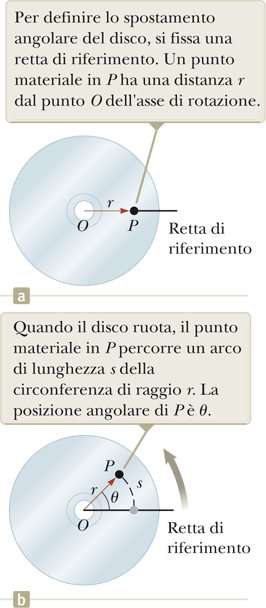
\includegraphics[width=0.25\textwidth]{cd_rotazione_corpo_rigido.png}
\end{wrapfigure}
Il disco ruota attorno ad un \textbf{asse fisso perpendicolare} 
al piano della figura e passante per il \textbf{centro $O$} del disco stesso. 

Un elemento infinitesimo del disco, schematizzabile come un punto 
materiale localizzato nel \textbf{punto $P$}, si trova ad una certa \textbf{distanza $r$ dall’origine} e ruota intorno ad essa percorrendo un traiettoria 
circolare di \textbf{raggio $r$}.

Rappresentiamo la posizione del punto P in termini delle sue \textbf{coordinate polari} $(r, \theta)$. Durante la rotazione, il raggio $r$ rimane costante, mentre
l'angolo $\theta$ varia nel tempo.

Quando il punto materiale si muove lungo la circonferenza da un punto sulla retta di riferimento $(\theta = 0)$ al punto $P$, percorre un arco di lunghezza $s$ come mostrato in figura.
Tale arco è legato all'angolo $\theta$ dalla relazione
\begin{align*}
    s &= r \theta \\
    \theta &= \frac{s}{r}
\end{align*}
L'angolo $\theta$ è un \textbf{numero puro} e la sua unità di misura sono i \textbf{radianti}.

\paragraph{Posizione angolare}
Scegliamo un raggio vettore condotto dall’origine $O$ ad un punto arbitrariamente scelto del disco.
La \textbf{posizione angolare} del corpo rigido viene quindi definita come l’angolo $\theta$ tra tale raggio vettore e la retta di riferimento, spesso scelta come \emph{asse x}.

\paragraph{Spostamento angolare}
Quando un punto materiale del corpo rigido si muove da \emph{A} a \emph{B} in un intervallo di tempo $\Delta t$, il raggio vettore spazza un angolo $\Delta \theta$.
Questa quantità viene definita lo \textbf{spostamento angolare} del corpo:
\begin{equation*}
    \Delta \theta = \theta_f - \theta_i
\end{equation*}

\paragraph{Velocità angolare}
La rapidità con cui avviene la rotazione può essere quantificata introducendo la \textbf{velocità angolare media} $\omega_{media}$ definita come il rapporto tra 
lo spostamento angolare $\Delta \theta$ e l'intervallo di tempo $\Delta t$ impiegato
\begin{equation*}
    \omega_{media} \equiv \frac{\theta_f - \theta_i}{t_f - t_i} = \frac{\Delta \theta}{\Delta t}
\end{equation*}
La \textbf{velocità angolare istantanea} è analogamente definita come il limite per $\Delta t \to 0$ della velocità angolare media:
\begin{equation*}
    \omega \equiv \lim_{\Delta t \to 0} \frac{\Delta \omega}{\Delta t} = \frac{d\omega}{dt}
\end{equation*}
La velocità angolare si misura in $rad/s$, o meglio in secondi$^{-1}$ ($s^{-1}$) essendo il radiante adimensionale.

La velocità angolare è positiva se l'angolo $\theta$ aumenta, ovvero quando il moto è in senso antiorario. Se l'angolo $\theta$ diminuisce, quindi il moto è
in senso antiorario, allora la velocità angolare sarà negativa.

\paragraph{Accelerazione angolare}
L’\textbf{accelerazione angolare media} $\alpha_{media}$ di un corpo in rotazione è il rapporto fra la variazione della velocità angolare e l’intervallo di tempo $\delta t$, in cui avviene tale variazione:
\begin{equation*}
    \alpha_{media} \equiv \frac{\omega_f - \omega_i}{t_f - t_i} = \frac{\Delta \omega}{\Delta t}
\end{equation*}
Analogamente, l'\textbf{accelerazione angolare istantanea} è il limite per $\Delta t \to 0$ dell'accelerazione angolare media:
\begin{equation*}
    \alpha \equiv \lim_{\Delta t \to 0} \frac{\Delta \omega}{\Delta t} = \frac{d\omega}{dt}
\end{equation*}
L’accelerazione angolare si misura in radianti per secondo al quadrato ($rad/s^{2}$), oppure in secondi$^{-2}$ ($s^{-2}$).

Si noti che alpha è positiva quando un corpo rigido che sta compiendo una rotazione antioraria ruota più rapidamente o, equivalentemente, quando un corpo rigido che sta compiendo una rotazione oraria ruota meno rapidamente.

Nel caso delle rotazioni intorno ad un asse fisso, tutti i punti materiali di un corpo rigido ruotano dello \textbf{stesso angolo} in un dato intervallo di tempo e quindi hanno la \textbf{stessa} \textbf{velocità angolare} e la \textbf{stessa accelerazione angolare}. 
Ciò significa che le grandezze $\theta$, $\omega$ ed $\alpha$ caratterizzano il moto rotatorio di tutto il corpo rigido così come quello di ogni sua parte.

\subsection{Corpo rigido con accelerazione costante}
Come nel caso del punto materiale abbiamo introdotto il modello di analisi punto materiale con accelerazione costante, ora introduciamo un nuovo 
modello di analisi chiamato \textbf{corpo rigido in moto con accelerazione angolare costante}.
Le leggi cinematiche che si applicano a tale modello, sono del tutto analoghe a quelle del moto rettilineo uniformemente accelerato:
\begin{align*}
    \omega_f &= \omega_i + \alpha t \\
    \theta_f &= \theta_i + \omega_i t + \tfrac{1}{2} \alpha t^2 \\ 
    \omega_f^2 &= \omega_i^2 + 2\alpha (\theta_f - \theta_i) \\
    \theta_f &= \theta_i + \tfrac{1}{2}(\omega_i + \omega_f) t
\end{align*}

\subsection{Variabili angolari e variabili linerari}
Vediamo ora le \textbf{relazioni} che legano la velocità angolare e l'accelerazione angolare di un corpo rigido in rotazione rispettivamente
alla velocità e all'accelerazione di un suo qualunque punto.
\begin{equation*}
    \text{Velocità tangenziale: } v_t = r\omega
\end{equation*}
\begin{equation*}
    \text{Accelerazione tangenziale: } a_t = r\alpha
\end{equation*}
\begin{equation*}
    \text{Accelerazione centripeta: } a_c = \tfrac{v^2}{r} = r\omega^2
\end{equation*}
L'accelerazione del punto sarà quindi uguale a
\begin{equation*}
    a = \sqrt{a_t^2 + a_c^2} = \sqrt{r^2\alpha^2 + r^2\omega^4} = r\sqrt{\alpha^2 + \omega^4}
\end{equation*}

\section{Momento di una forza}
Valutiamo il sistema rappresentato in figura, in cui una chiave inglese viene usata per serrare il dado; dado e chiave possono ruotare intorno ad un asse, 
perpendicolare al piano della figura.
\begin{figure}[h]
    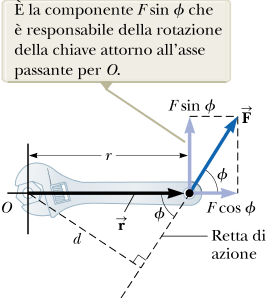
\includegraphics[scale=0.4]{momento_forza.png}
    \centering
\end{figure}

In generale, la forza $\vec{F}$ forma un angolo $\phi$ con la chiave. Definiamo il modulo del momento della forza $\vec{F}$ attorno all’asse passante per $O$ tramite la relazione
\begin{equation*}
    \tau \equiv r F \sin{\phi} = F d
\end{equation*}
dove $r$ rappresenta la distanza fra l’asse di rotazione ed il punto di applicazione della forza $\vec{F}$ e $d$ è la distanza fra l’asse di rotazione e la retta di azione della forza $\vec{F}$.

È facilmente ricavabile che 
\begin{equation*}
    d = r sin \phi
\end{equation*}
Questa grandezza viene chiamata \textbf{braccio} della forza $\vec{F}$.

Si noti che $\tau$ è massimo per un angolo $\phi$ di 90°, cioè quando la forza $\vec{F}$ è applicata perpendicolarmente a $r$. Quando invece la forza viene applicata
parallelamente a $r$, il momento è nullo.

Convenzione sul segno del momento:
\begin{itemize}
    \item Il momento della forza è positivo se la forza tende a far ruotare il corpo in senso antiorario
    \item Il momento della forza è positivo se la forza tende a far ruotare il corpo in senso orario
\end{itemize}

\subsection{Prodotto vettoriale}
Dati due vettori $\vec{A}$ e $\vec{B}$ si definisce il prodotto vettoriale tra $\vec{A}$ e $\vec{B}$ con il vettore $\vec{C}$ così definito:
\begin{align*}
    C &= A \times B \\
    C &\equiv AB \sin{\theta}
\end{align*}
la direzione del vettore C è perpendicolare al piano individuato da A e B. Per il segno si utilizza la regola della mano destra: le dita parallele al vettore A vanno chiuse verso il vettore B; il pollice indicherà il verso.

Alcune proprietà del prodotto vettoriale:
\begin{itemize}
    \item Il prodotto vettoriale non è commutativo: $A \times B = -B \times A$
    \item Se $A \parallel B$, allora $A \times B = 0$
    \item Se $A \bot B$, allora $\abs*{A \times B} = AB$
    \item Proprietà distributiva: $A \times (B + C) = A \times B + A \times C$
    \item Derivata: $\tfrac{d}{dt}(A \times B) = \tfrac{dA}{dt} \times B + A \tfrac{dB}{dt}$
\end{itemize}

\paragraph{Momento come prodotto vettoriale}
Il momento di una forza può essere espresso come il prodotto vettoriale tra $\vec{r}$ e $\vec{F}$
\begin{equation*}
    \tau \equiv r \times F
\end{equation*}

\subsection{Corpo rigido soggetto a un momento risultante}
Si consideri un punto materiale di massa $m$ che si muove lungo una circonferenza di raggio $r$ 
sotto l’azione di una risultante tangenziale delle forze $\sum \vec{F}_t$ e di una risultante radiale $\sum \vec{F}_r$.

La componente radiale è responsabile dell'accelerazione centripeta e ha momento nullo rispetto al centro della circonferenza, essendo antiparallela. 

La forza tangenziale è responsabile dell'accelerazione tangenziale $\vec{a}_t$, ovvero il cambiamento del modulo della velocità, e in base alla seconda legge
della dinamica abbiamo che 
\begin{equation*}
    \sum \vec{F}_t = ma_t
\end{equation*}
Moltiplicando entrambi i termini per il raggio $r$, e tenendo a mente che essendo la forza tangenziale \emph{perpendicolare}, il $\sin$ di $\theta$ è nullo, possiamo scrivere
\begin{equation*}
    \sum \tau = \sum F_t r = (ma_t) r
\end{equation*}
A questo punto, avendo definito in precedenza $a_t = r\alpha$, possiamo riscrivere la precedente equazione
\begin{equation*}
    \sum \tau = (mr\alpha)r = (mr^2)\alpha
\end{equation*}
Definiamo ora \textbf{\emph{I}} come la quantità $mr^2$, che chiameremo \textbf{\emph{Momento d'Inerzia}}.
Questo ci consente di riscrivere nuovamente la precedente equazione
\begin{equation*}
    \sum \tau \equiv I\alpha
\end{equation*}
Notiamo che questa formula ha la stessa forma della seconda legge di Newton $\sum F = ma $.

Estendiamo lo stesso ragionamento al caso di un \emph{corpo rigido di forma arbitraria}, che ruota intorno ad un asse fisso passante per $O$.
Il corpo può essere considerato come un insieme di punti materiali di massa $m_i$.

Per ogni elemento, in base alla seconda legge di Newton si ha:
\begin{equation*}
    F_i = m_i a_i
\end{equation*}
Il momento associato ad ogni forza rispetto all'asse di rotazione è
\begin{equation*}
    \tau_i = r_i F_i = r_i m_i a_i 
\end{equation*} 
Essendo $a_i = r_i\alpha$, possiamo scrivere 
\begin{equation*}
    \tau_i = m_i r_i^2 \alpha
\end{equation*}
È importante ricordare che, sebbene ogni punto materiale del corpo rigido abbia una accelerazione ai diversa, \textbf{l’accelerazione 
angolare} \textbf{$\alpha$} \textbf{è la stessa per tutti i punti}.
Tenendo presente questo fatto è possibile sommare i momenti agenti su ciascuno dei punti materiali che costituiscono il corpo rigido 
per ottenere il \textbf{momento risultante} rispetto ad un asse passante per $O$ e \emph{dovuto a tutte le forze esterne agenti sul corpo}:
\begin{equation*}
    \sum \tau_{est} = \sum_i \tau_i = \sum_i m_ir_i^2\alpha = \left( \sum_i m_ir_i^2 \right) \alpha = I\alpha
\end{equation*}
Otteniamo la formulazione matematica del modello \textbf{corpo rigido soggetto a un momento risultante}, che è l'\emph{analogo rotazionale} del modello 
\emph{punto materiale soggetto ad una forza risultante}.

\subsection{Calcolo dei momenti di Inerzia}
Dalla precedente relazione abbiamo definito il \emph{momento di inerzia} con la seguente equazione
\begin{equation*}
    I = \sum_i m_ir_i^2
\end{equation*}
Immaginando che il corpo sia suddiviso in tanti piccoli elementi di volume, ciascuno di massa $\Delta m_i$ abbiamo
definizione di momento di Inerzia per un corpo esteso
\begin{equation*}
    I = \sum_i r_i^2 \Delta m_i    
\end{equation*}
passando al limite per $m_i \to 0$ la somma diventa un integrale esteso a tutto il corpo rigido
\begin{equation*}
    I = \lim_{\Delta m_i \to 0} \sum_i r_i^2 \Delta m_i = \int r^2 dm
\end{equation*}

È di solito più facile calcolare i momenti d’inerzia in termini di elementi di volume piuttosto che in termini delle loro masse.
Questo si può fare usando la densità $\rho \equiv m/V$. Ricaviamo quindi $dm = \rho dV$
\begin{equation*}
    I = \int \rho r^2 dV
\end{equation*}
Il momento d'inerzia varia cambiando la posizione dell'asse di rotazione.

\paragraph{Teorema degli assi peralleli} Se il momento d'Inerzia di un corpo calcolato rispetto ad un asse passante per il suo centro di massa è $I_{CM}$, il momento d'Inerzia
calcolato dispetto ad un qualunque altro asse (parallelo al primo) e distante $D$ rispetto da esso, vale:
\begin{equation*}
    I = I_{CM} + MD^2
\end{equation*}

\subsection{Energia cinetica di rotazione}
Consideriamo quindi un corpo rigido come un insieme di punti materiali ed assumiamo che esso sia in moto rotatorio attorno ad un asse fisso
$z$ con una velocità angolare $\omega$.
Valutiamo un punto materiale posizionato a distanza $r_i$ dall'asse di rotazione. Indicando con $m_i$ la massa del punto materiale e con
$v_i$ la sua velocità, l'energia cinetica di tale punto materiale è
\begin{equation*}
    K_i = \tfrac{1}{2} m_i v_i^2
\end{equation*}
Ricordando che ogni punto materiale del corpo ha la stessa velocità angolare $\omega$ e che la velocità dei singoli punti dipende dalla loro distanza $r_i$
dall'asse di rotazione, l'energia cinetica totale del corpo rigido non è altro che la somma delle energie cinetiche dei singoli
punti materiali che lo compongono
\begin{equation*}
    K_R = \sum_i K_k = \sum_i \tfrac{1}{2} m_i v_i^2 = \tfrac{1}{2} \sum_i m_i r_i^2 \omega^2
\end{equation*}
Che possiamo scrivere anche nella forma
\begin{equation*}
    K_R = \tfrac{1}{2} \left(\sum_i m_i r_i^2 \right) \omega^2
\end{equation*}
Riconosciamo quindi che $\omega^2$ è uguale per tutti i punti e che la quantità dentro le parentesi è il momento di inerzia del corpo:
\begin{equation*}
    K_R = \tfrac{1}{2} I \omega^2
\end{equation*}

\subsection{Considerazioni energetiche nel moto rotatorio}
Consideriamo il corpo rigido in figura che può ruotare intorno ad un asse passante per $O$ e supponiamo che la sola forza esterna $\vec{F}$ 
sia applicata nel punto $P$. 
\begin{figure}[h]
    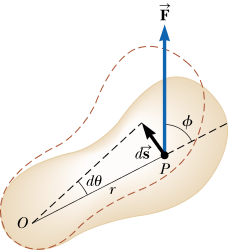
\includegraphics[scale=0.4]{lavoro_corpo_rotazione.png}
    \centering
\end{figure}
La forza $\vec{F}$ giace nel piano del foglio. Il lavoro compiuto da $\vec{F}$, quando il suo punto 
di applicazione ruota intorno all’asse di un tratto infinitesimo, $ds = r d \theta$ è
\begin{equation*}
    dW = \vec{F} \cdot d\vec{s} = (F \sin{\phi})r d\theta 
\end{equation*}
Poiché il modulo del momento intorno ad $O$ della forza $\vec{F}$ equivale a $rF \sin{\phi}$, possiamo riscrivere il lavoro come
\begin{equation*}
    dW = \tau d\theta
\end{equation*}

Il lavoro compiuto nell’unità di tempo si ottiene dividendo il lavoro della forza $\vec{F}$ applicata al corpo in rotazione 
per l’intervallo $dt$ in cui la forza ha agito
\begin{equation*}
    \frac{dW}{dt} = \tau \frac{d\theta}{dt}
\end{equation*}

La grandezza $dW/dt$ non è altro che la \textbf{potenza P} sviluppata dalla forza ed essendo $d\theta / dt = \omega$ l'equazione si riduce a
\begin{equation*}
    P = \frac{dW}{dt} = \tau \omega
\end{equation*}

\paragraph{Teorema del lavoro ed energia cinetica}
Analogamente al teorema lavoro-energia cinetica per il moto traslatorio, questo teorema 
afferma che il lavoro fatto dalla risultante delle forze esterne su un corpo rigido che ruota intorno ad 
un asse fisso è uguale alla variazione della energia cinetica di rotazione del corpo.
\begin{equation*}
    W = \int_{\omega_i}^{\omega_f} I\omega \; d\omega = \tfrac{1}{2} I\omega_f^2 - \tfrac{1}{2}I\omega_i^2
\end{equation*}

Se un corpo in rotazione è isolato e tutte le forze interne sono conservative, si può applicare il modello sistema isolato
e quindi il principio di conservazione dell’energia meccanica.

\section{Momento angolare}
Si consideri un punto materiale di massa $m$, a cui è associata la quantità di moto $\vec{p}$ e la cui posizione sia individuata dal vettore $\vec{r}$.
Nel descrivere il moto di traslazione di un punto materiale, abbiamo trovato che $\sum \vec{F} = \vec{p}/dt$.
Moltiplichiamo vettorialmente $r$ da entrambe le parti
\begin{equation*}
    \vec{r} \times \sum \vec{F} = \sum \vec{\tau} = \vec{r} \times \frac{d\vec{p}}{dt}
\end{equation*}
Aggiungiamo ora al termine di destra la quantità $\tfrac{d\vec{r}}{dt}\times \vec{p}$ che è uguale a zero in quanto $\tfrac{d\vec{r}}{dt} = \vec{v}$,
e i vettori $\vec{v}$ e $\vec{p}$ sono paralleli. Otteniamo quindi
\begin{equation*}
    \sum \vec{\tau} = \vec{r} \times \frac{d\vec{p}}{dt} + \frac{d\vec{r}}{dt}\times \vec{p}
\end{equation*}
che possiamo riscrivere come
\begin{equation*}
    \sum \vec{\tau} = \frac{d(\vec{r} \times \vec{p})}{dt}
\end{equation*}

\paragraph{Definizione}
Il \textbf{momento angolare} $\vec{L}$ di un punto materiale rispetto ad un asse passante per l’origine $O$ è, ad un certo istante, il prodotto vettoriale 
tra il vettore posizione $\vec{r}$ del punto materiale e la sua quantità di moto $\vec{p}$:
\begin{equation*}
    \vec{L} \equiv \vec{r} \times \vec{p}
\end{equation*}
Possiamo quindi riscrivere la precedente equazione come
\begin{equation*}
    \sum \vec{\tau} = \frac{d(\vec{r} \times \vec{p})}{dt} = \frac{d\vec{L}}{dt}
\end{equation*}

\subsection{Momento angolare di un corpo rigido in rotazione}
Restringiamo ora l’analisi su un corpo rigido in rotazione attorno ad un asse fisso coincidente con l’asse $z$ del sistema
di coordinate del quale vogliamo determinare il momento angolare. Tutti i punti materiali che costituiscono il corpo rigido 
ruotano nel piano $xy$, attorno all’asse $z$, con la stessa velocità angolare $\omega$. 

Il modulo del momento angolare intorno all’asse $z$ dell’i-esimo punto materiale di massa $m_i$ è $m_iv_ir_i$ e, poiché $v_i = r_i\omega$ si ha
\begin{equation*}
    L_i = m_ir_i^2 \omega
\end{equation*}

Siamo ora in grado di trovare il momento angolare totale del corpo (che, in questo caso ha solo componente nell'asse $z$)
effettuando la somma degli $L_i$ su tutti i punti materiali:
\begin{equation*}
    L_z = \sum_i L_i = \sum_i m_ir_i^2 \omega = \left(\sum_i m_ir_i^2 \right) \omega
\end{equation*}
da cui possiamo finalmente trovare che
\begin{equation*}
    L_z = I\omega
\end{equation*}
tale equazione è matematicamente simile all'equazione per la quantità di moto.

\subsection{Conservazione del momento angolare}
\paragraph{Definizione} 
Il \textbf{momento angolare totale} di un sistema \textbf{rimane costante} (in modulo, direzione e verso) se è \textbf{nullo} il \textbf{momento} 
\textbf{risultante} delle \textbf{forze esterne}, cioè se il \textbf{sistema} è \textbf{isolato}.

~\newline
Questo principio è alla base del modello sistema isolato basato sul momento angolare. Vediamo infatti che se risulta
\begin{equation*}
    \sum \vec{\tau}_{est} = \frac{d\vec{L}_{tot}}{dt} = 0
\end{equation*}
allora si ha
\begin{equation*}
    \Delta \vec{L}_{tot} = 0
\end{equation*}

Nel caso in cui durante il moto rotatorio la distribuzione delle masse di un corpo materiale si modifichi, il suo momento 
di inerzia cambia nel tempo; necessariamente, poiché il modulo del momento angolare del sistema è $L = I\omega$, la conservazione
del momento angolare implica che il prodotto di $I$ per $\omega$ rimanga costante. Pertanto, se il sistema è isolato, ad una variazione di
$I$ deve corrispondere una variazione di $\omega$. In questo caso, scriveremo il principio di conservazione del momento angolare come
\begin{equation*}
    I_i\omega_i = I_f\omega_f = \text{costante}
\end{equation*}

\subsection{Moto di giroscopi e trottole}
Nel moto di rotazione della trottola abbiamo due diverse rotazioni: la rotazione della trottola intorno al suo asse e la rotazione dell'asse della trottola
intorno ad un asse verticale, ovvero l'asse $z$.

La trottola è soggetta alla forza peso applicata al suo centro di massa e dovrebbe cadere se non fosse in rotazione, ovvero se non possedesse momento angolare.

Il moto dell’asse di simmetria attorno alla verticale è detto \textbf{moto di precessione} ed è generalmente più lento rispetto al moto di rotazione della trottola intorno al proprio asse.

Ll centro di massa della trottola non si trova sulla verticale del punto di appoggio $O$ e, quindi, rispetto a questo punto, la forza peso $M\vec{g}$ della 
trottola ha un momento, che farebbe certamente cadere la trottola se questa non fosse in rotazione. A causa del moto di rotazione, la trottola possiede un momento angolare $\vec{L}$ diretto lungo il suo asse di simmetria.

Le caratteristiche fondamentali del moto di precessione possono essere illustrate considerando il semplice \textbf{giroscopio} mostrato in figura.
Mentre la reazione vincolare ha momento nullo, la forza peso $M\vec{g}$ rivolta verso il basso ha un momento dato da $\vec{\tau} = \vec{r} \times M \vec{g}$.
Sappiamo già che il momento della forza applicata produce un cambiamento del momento angolare, ovvero $\tau = \tfrac{d\vec{L}}{dt}$.
\begin{figure}[h]
    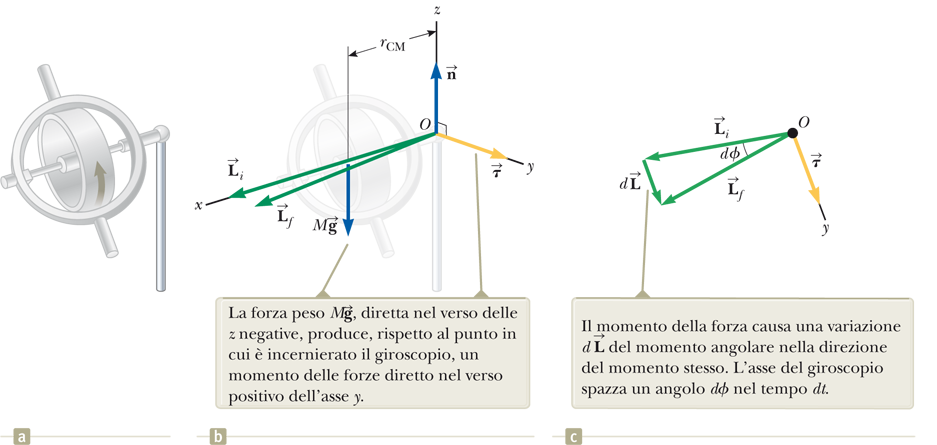
\includegraphics[scale=0.6]{giroscopio_momento.png}
    \centering
\end{figure}

Si osserva che il momento $\vec{\tau}$ produce nell’intervallo di tempo $dt$ una variazione di momento angolare $d\vec{L}$ che ha la stessa direzione e 
verso di $\vec{\tau}$ , ed è quindi perpendicolare a $\vec{L}$. In un intervallo di tempo, la variazione del momento angolare è $d\vec{L} = \vec{L}_f - \vec{L}_i = \vec{\tau}dt$.
Poiché $d\vec{L}$ è perpendicolare a $\vec{L}$, il modulo di $\vec{L}$ non cambia, ma cambia la sua direzione: ha la stessa direzione e verso di $\vec{\tau}$.





\end{document}
